%!TEX root=./LIVRO.tex
\addcontentsline{toc}{chapter}{SIMULADO 1}
\markboth{Simulado 1}{}

\num{1} OBSERVE OS AGRUPAMENTOS A SEGUIR.

\begin{figure}[H]
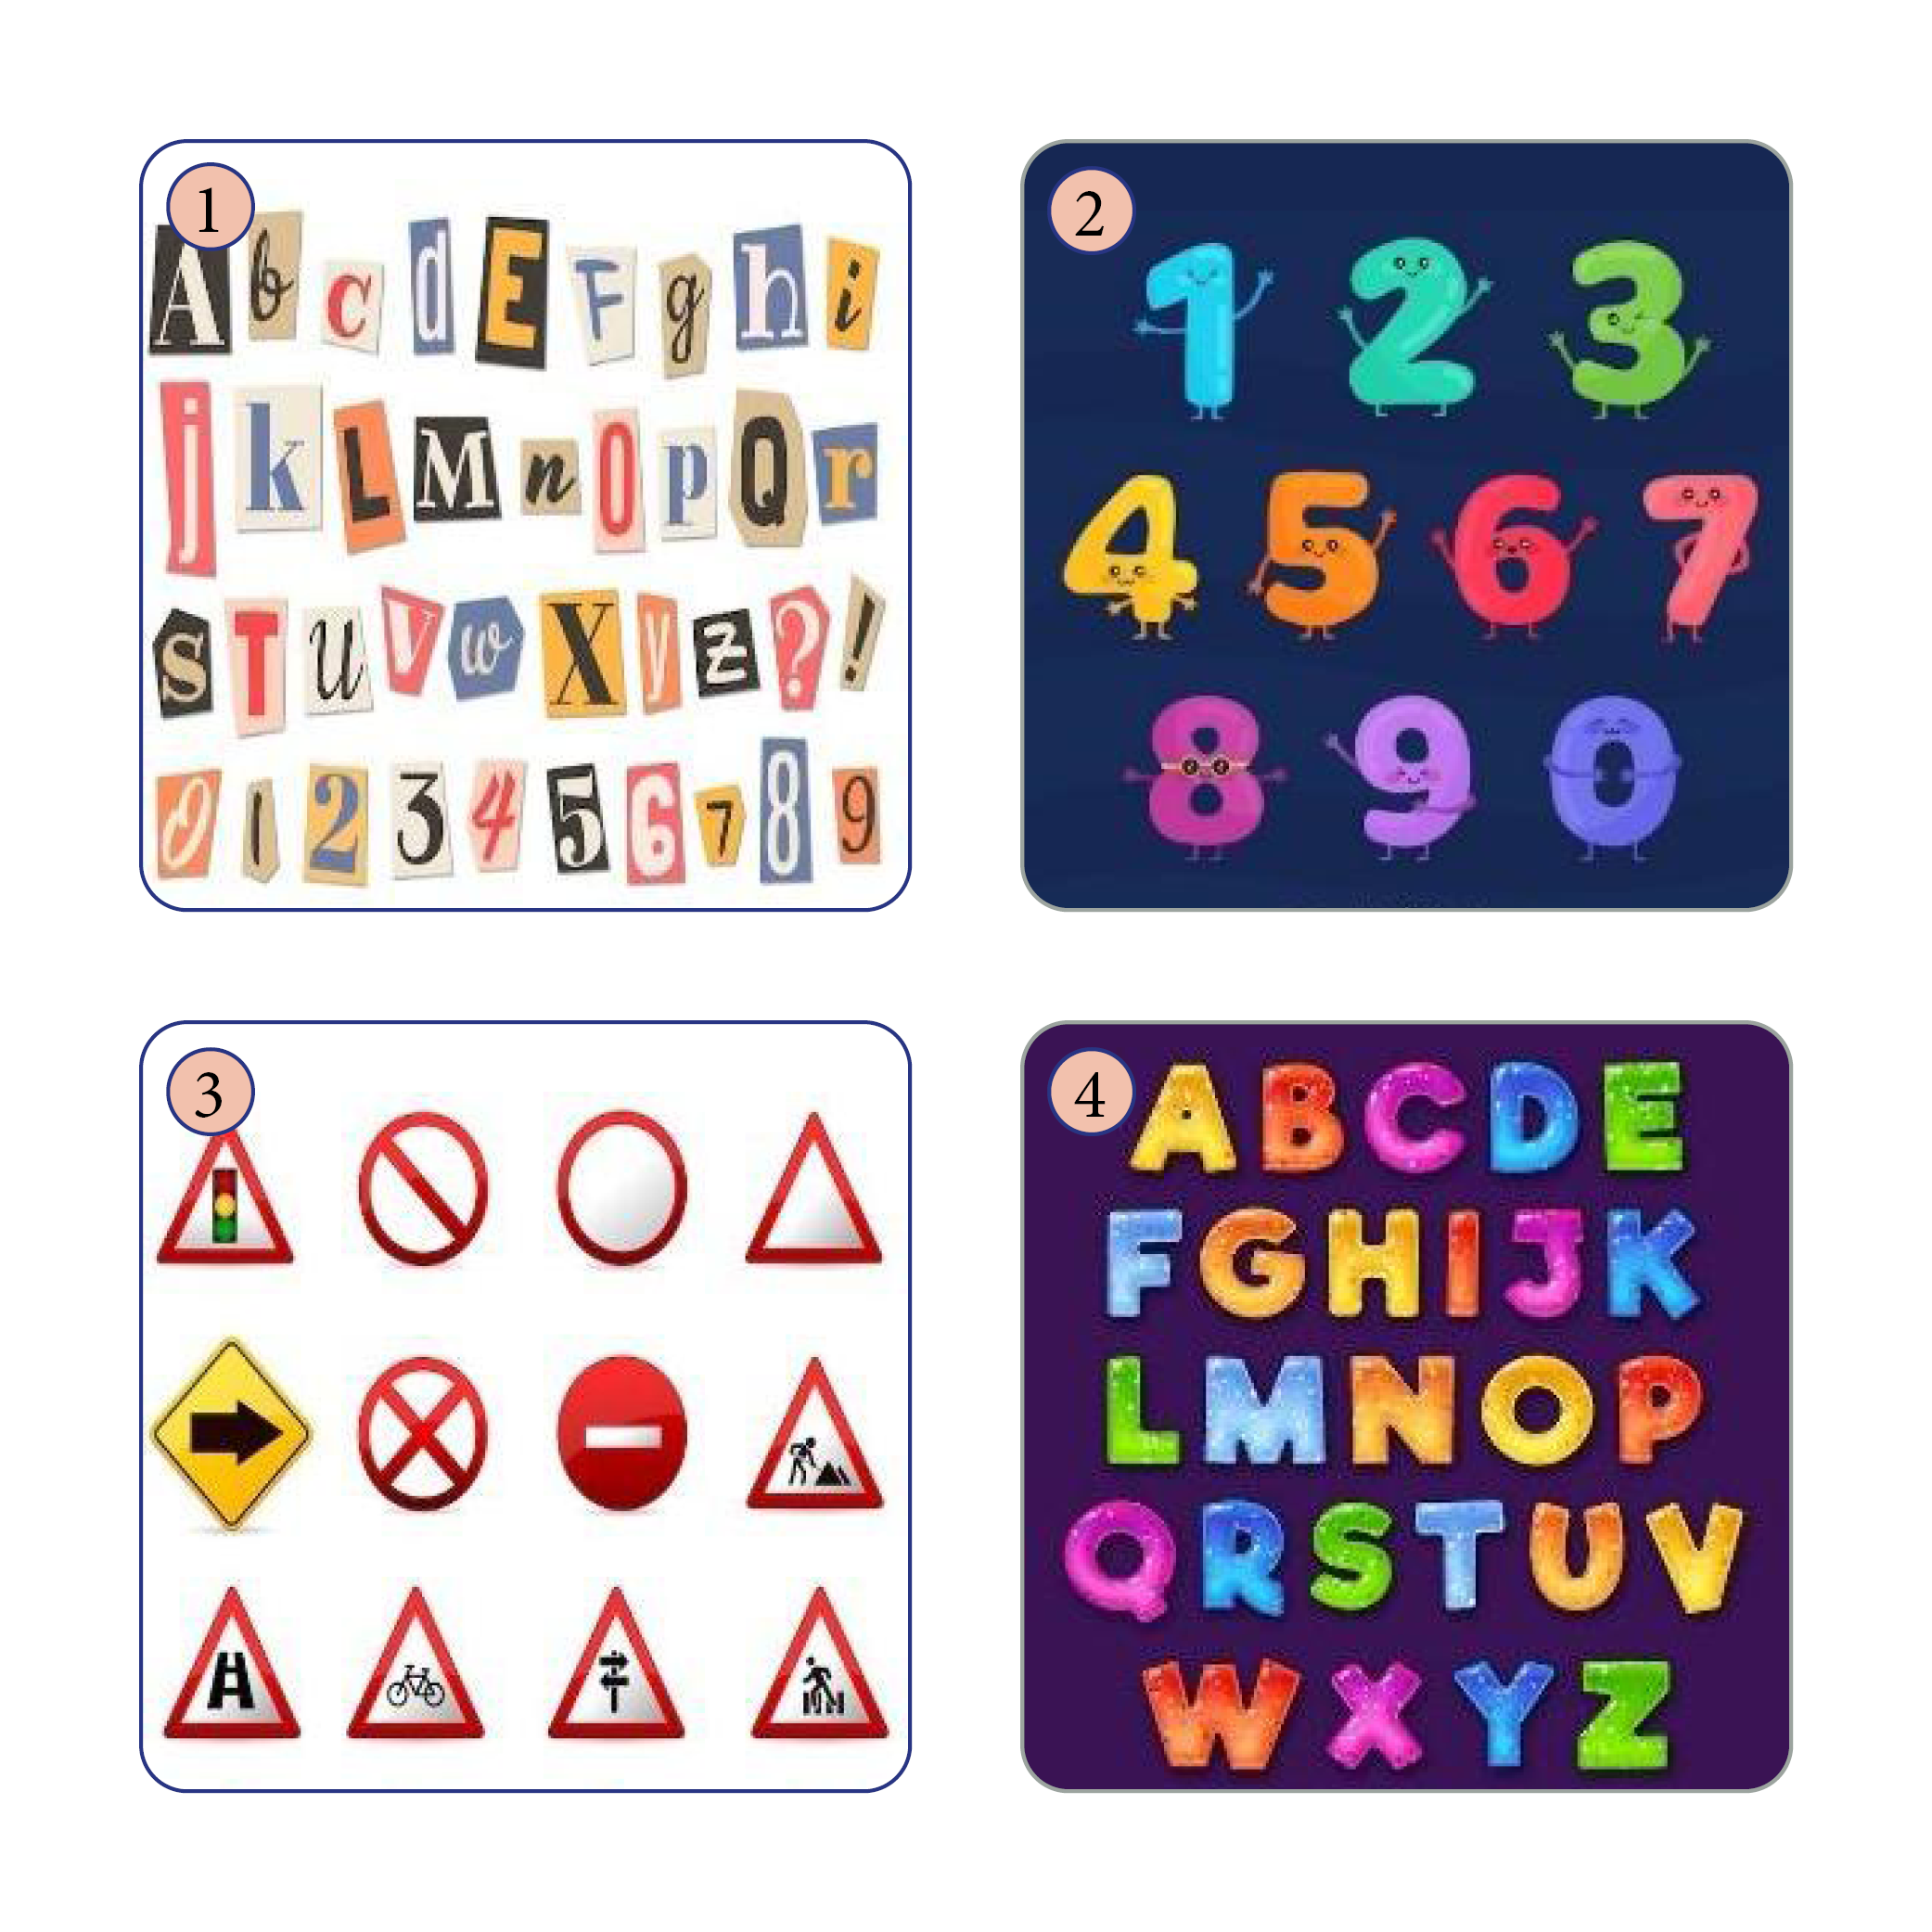
\includegraphics[width=\textwidth]{media/image183a186}
\end{figure}

O AGRUPAMENTO EM QUE SÓ APARECEM LETRAS É O

\begin{multicols}{2}
\begin{escolha}
\item SUPERIOR ESQUERDO.

\item SUPERIOR DIREITO.

\item INFERIOR ESQUERDO.

\item INFERIOR DIREITO.
\end{escolha}
\end{multicols}

\pagebreak
\num{2} VEJA O ANIMAL DE ESTIMAÇÃO QUE DANIEL GANHOU.

\begin{figure}[htpb!]
\centering
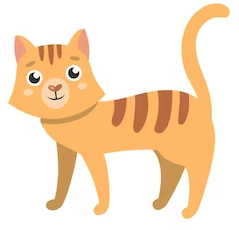
\includegraphics[width=.4\textwidth]{media/image187.png}
\end{figure}

A LETRA INICIAL DO NOME DO ANIMAL É 

\begin{escolha}
\item R.

\item P.

\item G .

\item K.
\end{escolha}

\num{3} OBSERVE A PALAVRA QUE JOÃO ESCREVEU NO PAPEL.

\begin{myquote}
BOLA
\end{myquote}

QUAL PALAVRA TEM A MESMA QUANTIDADE DE SONS? 

\begin{escolha}
\item MACACO.

\item BONECA.

\item PATINETE.

\item PIPA.
\end{escolha}

\pagebreak
\num{4} VEJA O TÊNIS QUE MATEUS GANHOU DA VOVÓ. 

\begin{figure}[htpb!]
\centering
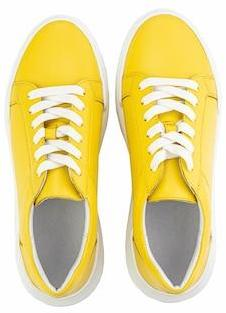
\includegraphics[width=.2\textwidth]{media/image189.jpg}
\end{figure}

QUAL É A SÍLABA FINAL DO NOME DA COR DO TÊNIS QUE MATEUS GANHOU?

\begin{escolha}
\item MA.

\item RE.

\item LO.

\item LU.
\end{escolha}

\num{5} VEJA A PALAVRA QUE JÚLIA LEU PARA SUA PRIMA.

\begin{myquote}
SALAME
\end{myquote}

QUAL PALAVRA TEM O MESMO O SOM DA SÍLABA MEDIAL DA PALAVRA QUE JÚLIA LEU?

\begin{escolha}
\item SALADA.

\item SACOLA.

\item LÂMPADA.

\item PANELA.
\end{escolha}

\pagebreak
\num{6} VEJA O PRESENTE QUE TOMAS GANHOU DO SEU AMIGO.

\begin{figure}[htpb!]
\centering
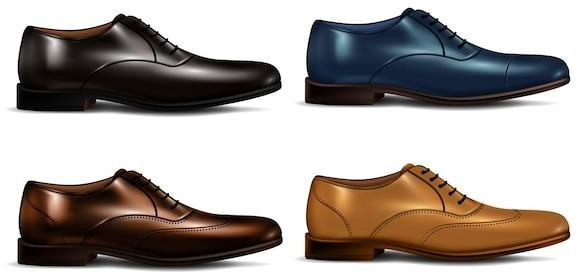
\includegraphics[width=.5\textwidth]{media/image191.jpg}
\end{figure}

O NOME DO PRESENTE QUE TOMAS GANHOU É

\begin{escolha}
\item SALADA.

\item SAPATO.

\item TOMATE.

\item PANELA.
\end{escolha}

\num{7} OBSERVE A FRUTA PREFERIDA DE SOFIA.

\begin{figure}[htpb!]
\centering
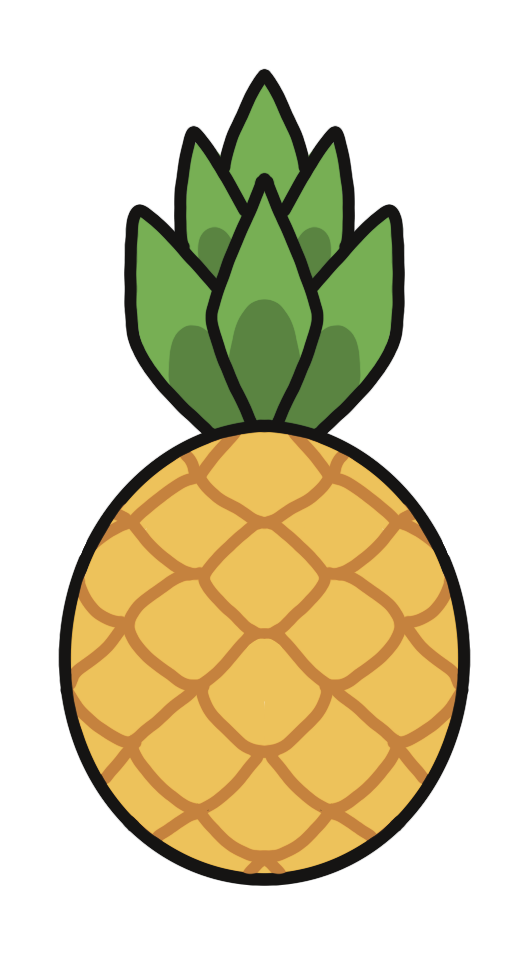
\includegraphics[width=.2\textwidth]{media/image192.png}
\end{figure}

ASSINALE O NOME CORRETO DESSA FRUTA.

\begin{escolha}
\item ABACAXI

\item ABXICA

\item ACAXI

\item ABACAI
\end{escolha}

\pagebreak
\num{8} VEJA A PALAVRA QUE GUTO ESCREVEU.

\begin{myquote}
TAPETE
\end{myquote}

A PALAVRA QUE TERMINA COM O MESMO SOM É

\begin{escolha}
\item GILETE.

\item PETECA.

\item TESOURA.

\item TAMANCO.
\end{escolha}

\num{9} LEIA ESSA FRASE.

\begin{myquote}
O MENINO CHUTA A BOLA.
\end{myquote}

A IMAGEM QUE REPRESENTA O QUE ESTÁ ESCRITO NA FRASE É

\begin{escolha}
\item 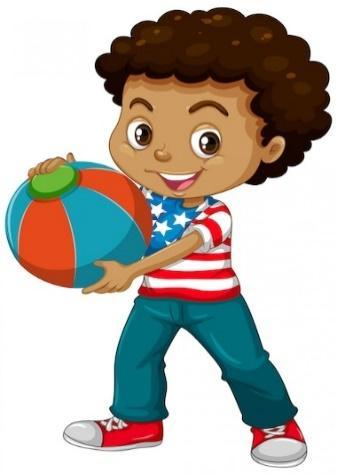
\includegraphics[width=.1\textwidth]{media/image199.jpg}

\item 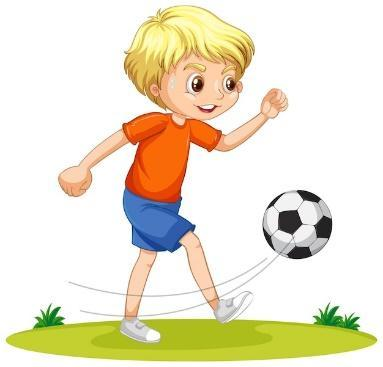
\includegraphics[width=.1\textwidth]{media/image200.jpg}

\item 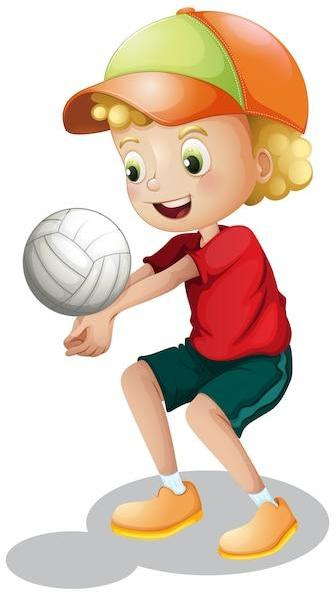
\includegraphics[width=.1\textwidth]{media/image201.jpg}

\item 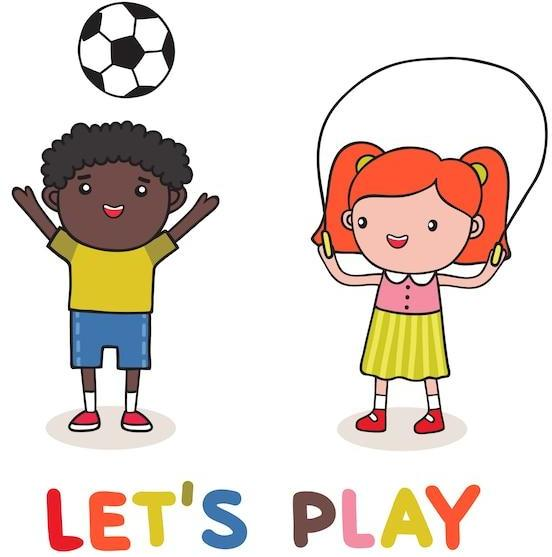
\includegraphics[width=.1\textwidth]{media/image202.jpg}
\end{escolha}

\num{10}

\begin{quote}
\begin{verse}
\textbf{O MEU CHAPÉU}

O MEU CHAPÉU TEM TRÊS PONTAS\\
TEM TRÊS PONTAS O MEU CHAPÉU.\\
SE NÃO TIVESSE TRÊS PONTAS\\
NÃO SERIA O MEU CHAPÉU.
\end{verse}

\fonte{Domínio Público. ADIVINHAS, CANÇÕES, CANTIGAS DE RODA, PARLENDAS, POEMAS, QUADRINHAS E TRAVA-LÍNGUAS. Disponível em: \emph{http://www.dominiopublico.gov.br/download/texto/me000588.pdf}. Acesso em 14 abr. 2023.}
\end{quote}

O ASSUNTO DESSE TEXTO É

\begin{escolha}
\item DESCOBRIR A QUEM PERTENCE O CHAPÉU.

\item MOSTRAR QUE O CHAPÉU NÃO SERVE PARA COLOCAR SOBRE A CABEÇA.

\item MOSTRAR QUE O CHAPÉU TEM MAIS DO QUE TRÊS PONTAS.

\item DESCREVER AS CARACTERÍSTICAS DO CHAPÉU.
\end{escolha}


\num{11} LEIA O TEXTO:

\begin{quote}
\begin{verse}
\textbf{A SEMANA INTEIRA}

A SEGUNDA FOI À FEIRA\\
PRECISAVA DE FEIJÃO;\\
A TERÇA FOI À FEIRA\\
PRA COMPRAR UM PIMENTÃO;\\
A QUARTA FOI À FEIRA
\end{verse}
\end{quote}


\begin{quote}
\begin{verse}
PRA BUSCAR QUIABO E PÃO;\\
A QUINTA FOI À FEIRA,\\
POIS GOSTAVA DE AGRIÃO;\\
A SEXTA FOI A FEIRA,\\
TEM BANANA? TEM MAMÃO?\\
SÁBADO NÃO TEM FEIRA\\
E DOMINGO TAMBÉM NÃO.
\end{verse}

\begin{flushright}
SÉRGIO CAPARELLI
\end{flushright}
\end{quote}

%Disponível em:\textbf{\emph{\href{http://tinyurl.com/2b7fs26z. Acesso em: 18 fev. 2023. }}

EM QUAIS DIAS DA SEMANA PODEMOS COMPRAR PIMENTÃO E MAMÃO?

\begin{escolha}
\item SÁBADO E DOMINGO.

\item DOMINGO E TERÇA.

\item QUARTA E SÁBADO.

\item TERÇA E SEXTA.
\end{escolha}

\num{12} LARA VAI CONVIDAR ALICE PARA SEU ANIVERSÁRIO.

QUAL TEXTO ELA DEVE MANDAR PARA SUA AMIGA? 

\begin{escolha}
\item BILHETE.

\item CONVITE.

\item NOTÍCIA.

\item RECEITA.
\end{escolha}

\pagebreak
\num{13} VEJA O CARTAZ.

\begin{figure}[htpb!]
\centering
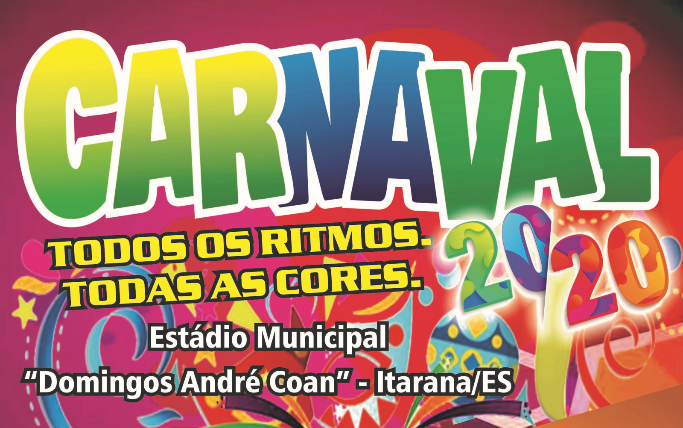
\includegraphics[width=\textwidth]{media/image204.png}
\end{figure}
%Disponível em:\href{https://www.itarana.es.gov.br/portal/artigo/prefeitura-municipal-de-itarana-apresenta-programacao-do-carnaval-2020-com-blocos-de-rua-e-shows-noturnos}{\emph{https://www.itarana.es.gov.br/portal/artigo/prefeitura-municipal-de-itarana-apresenta-programacao-do-carnaval-2020-com-blocos-de-rua-e-shows-noturnos}} Acesso em: 19 fev. 2023. 

ESSE TEXTO SERVE PARA

\begin{escolha}
\item ORGANIZAR TAREFAS.

\item ENSINAR UMA RECEITA.

\item ANUNCIAR UM EVENTO.

\item CONTAR UMA HISTÓRIA.
\end{escolha}

\num{14} LEIA O TRECHO DA HISTÓRIA DE JOÃO E MARIA.

\begin{quote}
NA MADRUGADA DO DIA SEGUINTE, A MADRASTA ACORDOU AS CRIANÇAS E FORAM
NOVAMENTE PARA A MATA. ENQUANTO CAMINHAVAM, JOÃOZINHO ESFARELOU TODO O
SEU PÃO E O DA IRMÃ, FAZENDO UMA TRILHA.
\end{quote}

\begin{quote}
DESSA VEZ SE AFASTARAM AINDA
MAIS DE CASA E, CHEGANDO A UMA CLAREIRA, OS PAIS DEIXARAM AS CRIANÇAS
COM A DESCULPA DE CORTAR LENHA, ABANDONANDO-AS. JOÃO E MARIA
ADORMECERAM, POR FOME E CANSAÇO E, QUANDO ACORDARAM, ESTAVA MUITO
ESCURO. MARIA DESATOU A CHORAR. MAS, DESTA VEZ, NÃO CONSEGUIRAM
ENCONTRAR O CAMINHO: OS PÁSSAROS DA MATA TINHAM COMIDO TODAS AS
MIGALHAS.

\fonte{Domínio Público. João e Maria. Disponível em: \emph: http://www.dominiopublico.gov.br/download/texto/me001614.pdf. Acesso em: 19 fev. 2023.}
\end{quote}

JOÃO FEZ A TRILHA DE PÃO PARA

\begin{escolha}
\item ALIMENTAR OS PASSARINHOS.

\item CONSEGUIR VOLTAR PARA CASA.

\item COMER QUANDO SENTISSE FOME.

\item FUGIR DO PAI E DA MADASTRA.
\end{escolha}

\num{15} OBSERVE O TEXTO E A IMAGEM:

\begin{minipage}{.3\textwidth}
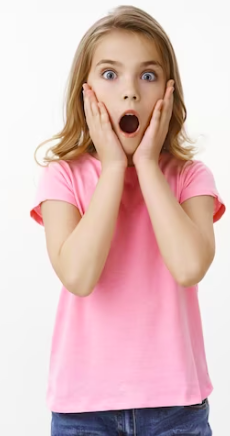
\includegraphics[width=\textwidth]{media/image205.png}
\end{minipage}
\begin{minipage}{.7\textwidth}
\begin{quote}
— NOSSA! ACABOU A LUZ! TENHO MEDO DO ESCURO!
\end{quote}

COMO A MENINA FICOU QUANDO FALTOU LUZ?

\begin{escolha}
\item TRISTE.

\item GRITANDO.

\item ASSUSTADA.

\item RECLAMANDO.
\end{escolha}
\end{minipage}

\pagebreak
% \vspace*{-4.2cm}
% \hspace*{-4cm}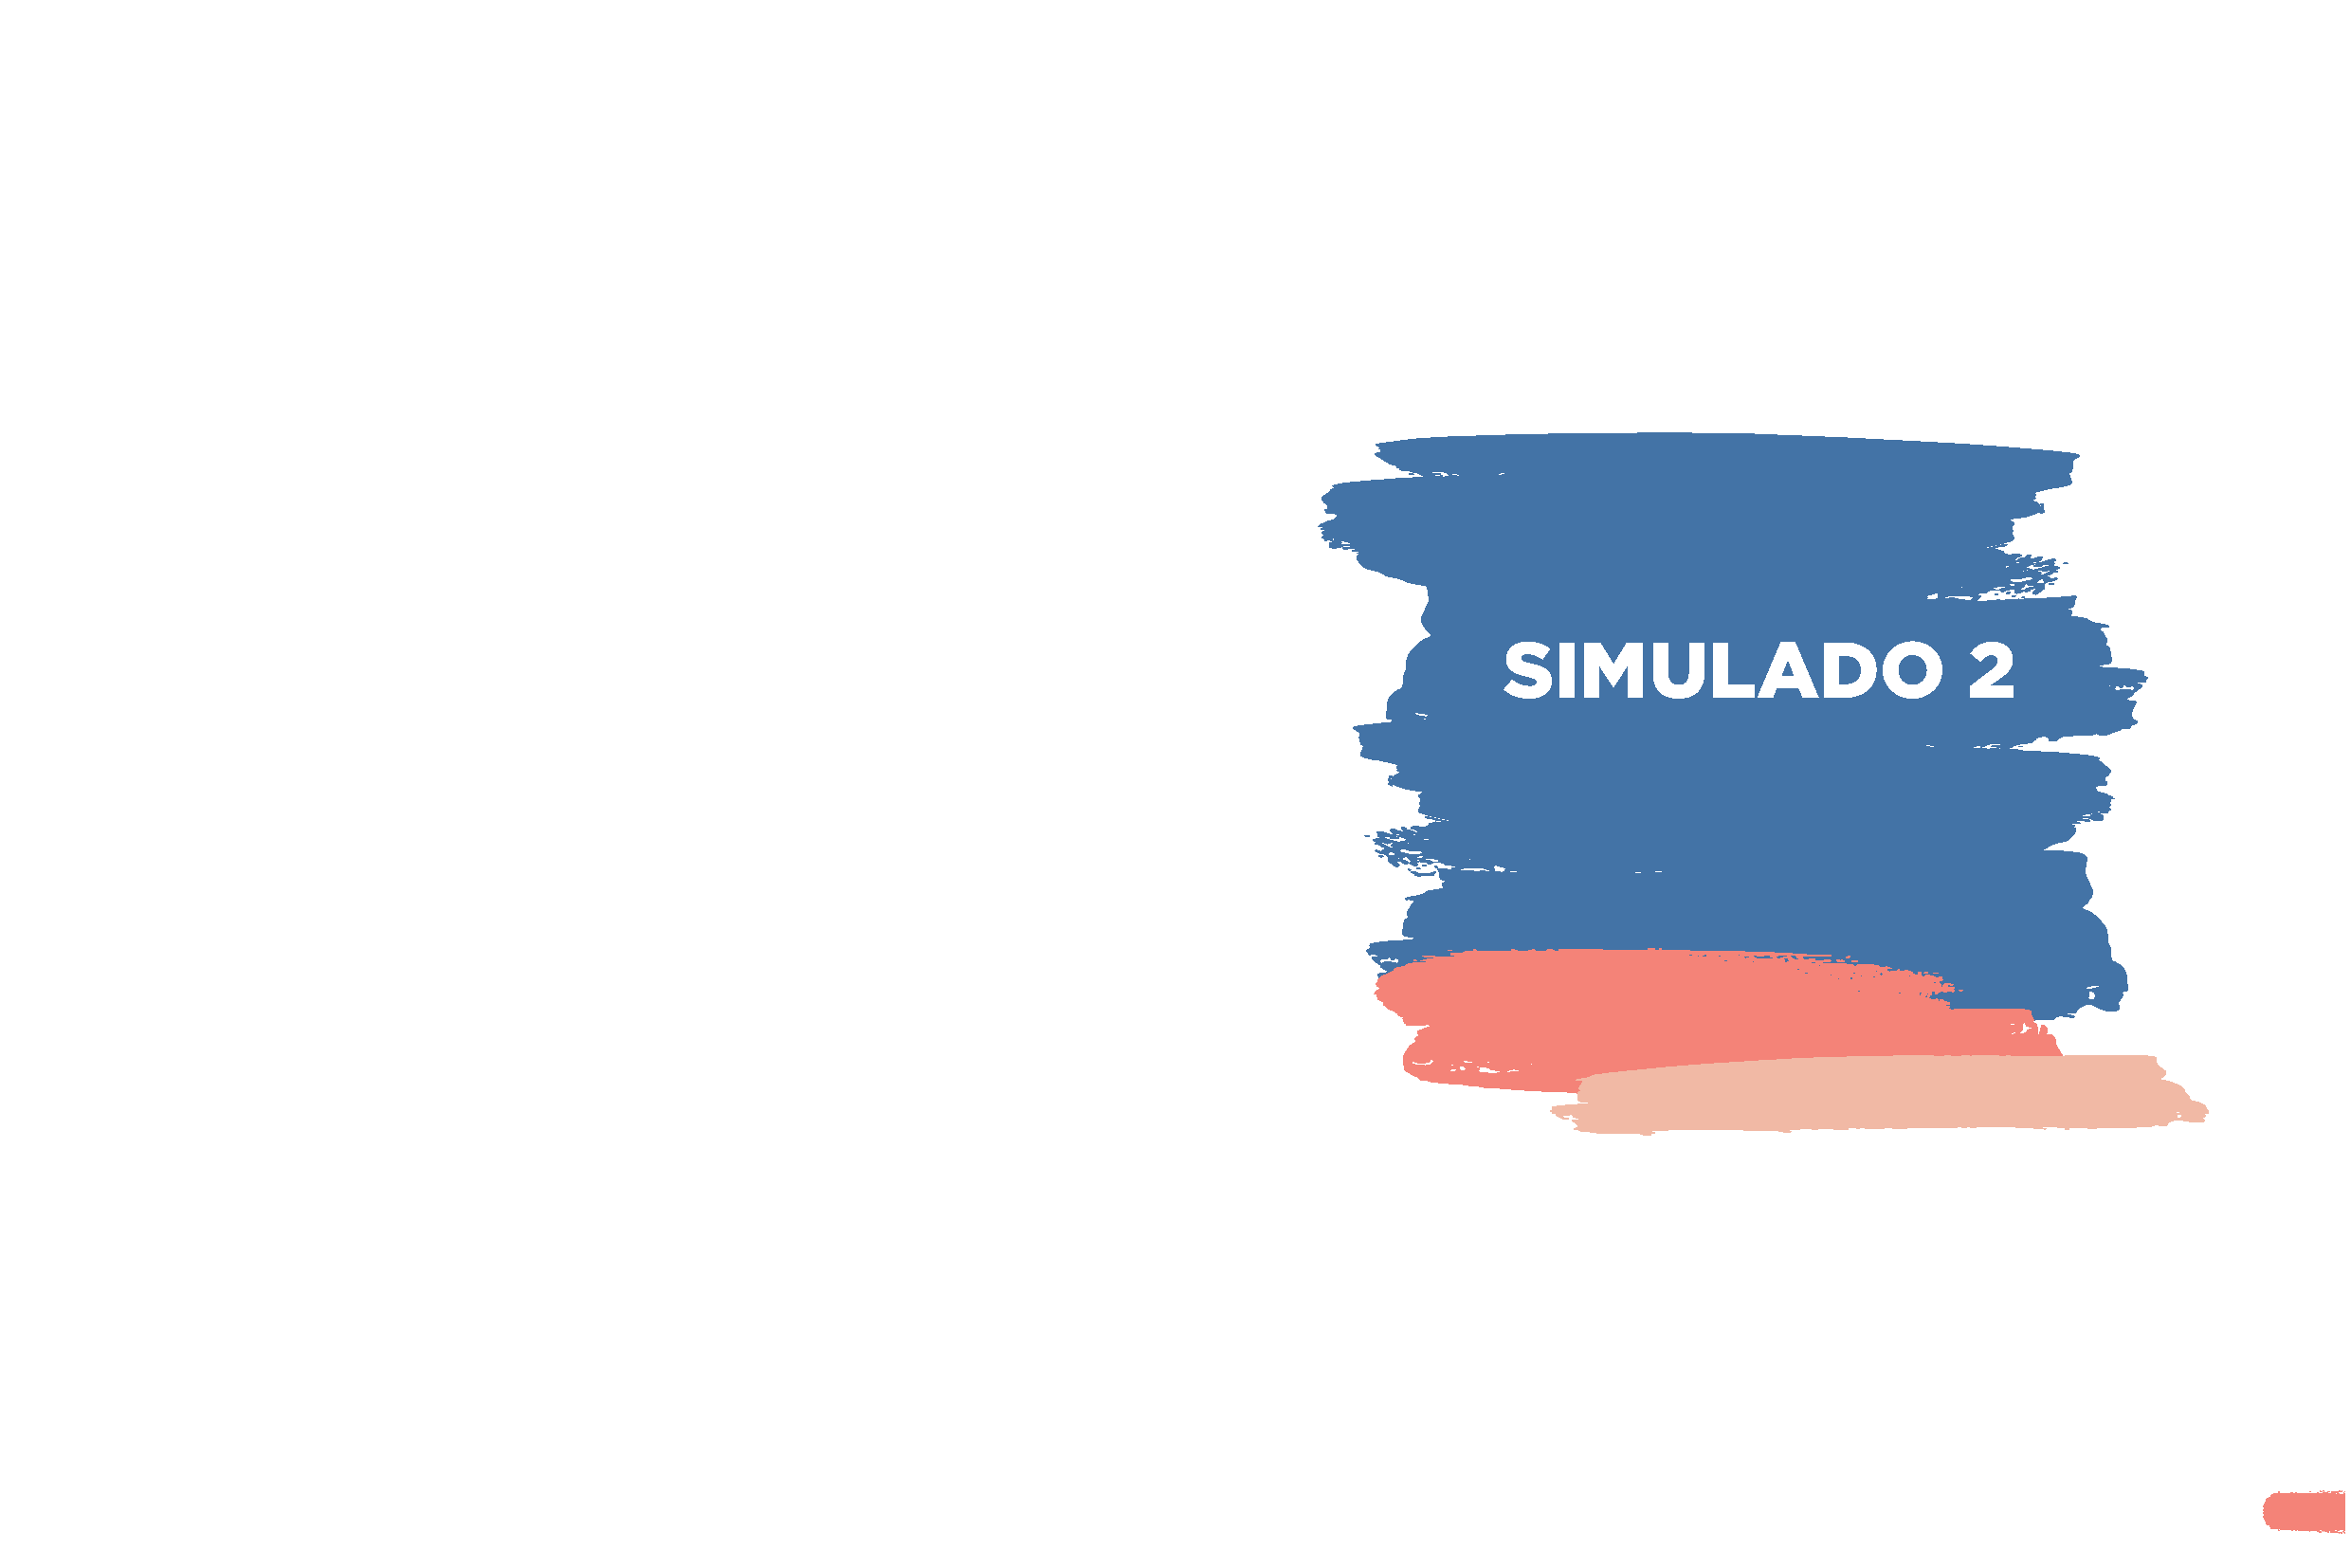
\includegraphics[scale=1]{../watermarks/2simulado5ano.pdf}

\addcontentsline{toc}{chapter}{SIMULADO 2}

\markboth{Simulado 2}{}

\pagebreak

\num{1} MARIANA QUER MOSTRAR PARA SUA AMIGA BIA QUE JÁ SABE ESCREVER O NOME DA SUA GATINHA MILU. PARA ISSO, ELA VAI ESCOLHER UMA MALETA DE SÍMBOLOS. 

\begin{figure}[htpb!]
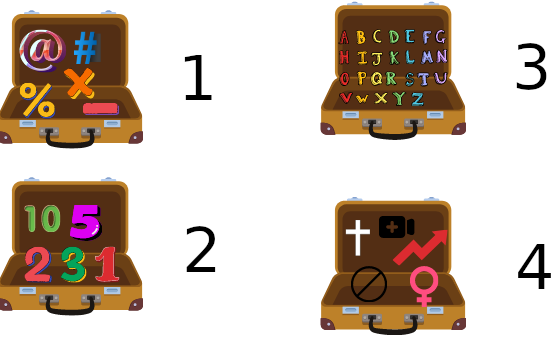
\includegraphics[width=\textwidth]{media/image209.png}
\end{figure}

QUAL MALETA MARIANA DEVE ESCOLHER?

\begin{escolha}
\item 1

\item 2

\item 3

\item 4
\end{escolha}

\num{2} OBSERVE O NOME DA FRUTA PREFERIDA DE ALICE.

\begin{figure}[htpb!]
\centering
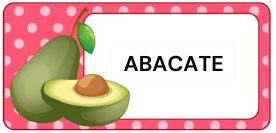
\includegraphics[width=.45\textwidth]{media/image212.png}
\end{figure}

\pagebreak
QUAL PALAVRA APRESENTA AS MESMAS VOGAIS INICIAIS E FINAIS DA FRUTA PREFERIDA DE ALICE?

\begin{escolha}
\item MACACO.

\item ÁRVORE.

\item COELHO.

\item GATO.
\end{escolha}


\num{3} OBSERVE A PALAVRA QUE ANA APRENDEU A LER.

\begin{myquote}
\textbf{FADA}
\end{myquote}

QUAL PALAVRA TEM A MESMA QUANTIDADE DE SONS?

\begin{escolha}
\item SALA.

\item TOMATE.

\item BONECA.

\item BICICLETA.
\end{escolha}


\num{4} MARINA JÁ CONSEGUE LER ALGUMAS PALAVRAS.

VEJA A PALAVRA QUE ELA LEU.

\begin{myquote}
\textbf{BONECA}
\end{myquote}

\pagebreak
AS LETRAS QUE FORMAM O SOM MEDIAL DA PALAVRA QUE ANA LEU SÃO

\begin{escolha}
\item B+O.

\item N+E.

\item C+A.

\item M+E.
\end{escolha}

\num{5} VEJA O ANIMAL DE ESTIMAÇÃO DE MIGUEL.

\begin{figure}[htpb]
\centering
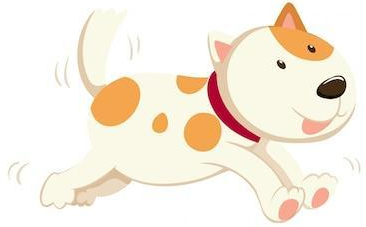
\includegraphics[width=.55\textwidth]{media/image214.jpg}
\end{figure}

A PALAVRA QUE COMEÇA COM A MESMA SÍLABA DO NOME DO ANIMAL É 

\begin{escolha}
\item CANECA.

\item BONECA.

\item CAVALO.

\item TUCANO.
\end{escolha}

\pagebreak
\num{6} VEJA O ANIMAL QUE TIAGO ADOTOU PARA ALEGRAR SUA FAZENDA.

\begin{figure}[htpb]
\centering
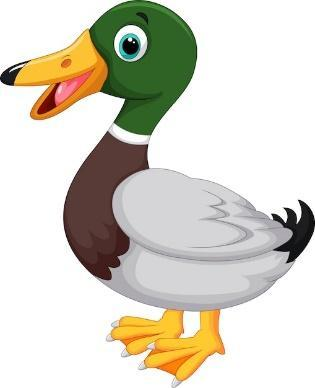
\includegraphics[width=.3\textwidth]{media/image215.jpg}
\end{figure}

A SÍLABA INICIAL DO NOME DESSE ANIMAL É

\begin{escolha}
\item GA.

\item TO.

\item BA.

\item PA.
\end{escolha}

\num{7} LEIA A PALAVRA ESCRITA NA PLACA.

\begin{myquote}
PANELA
\end{myquote}

A ÚLTIMA LETRA DESSA PALAVRA É

\begin{escolha}
\item P

\item N

\item E

\item A
\end{escolha}

\pagebreak

\num{8} OBSERVE O BRIQUEDO QUE MONIQUE COMPROU PARA SUA COLEÇÃO.

\begin{figure}[htpb]
\centering
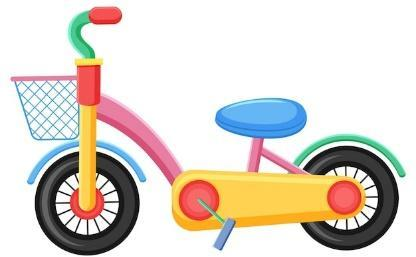
\includegraphics[width=.3\textwidth]{media/image217.jpg}
\end{figure}

O NOME DO BRINQUEDO QUE ELA COMPROU É

\begin{escolha}
\item BISCOITO.

\item BICICLETA.

\item TRICICOLO.

\item CANETA.
\end{escolha}

\num{9} OBSERVE A CENA.

\begin{figure}[htpb]
\centering
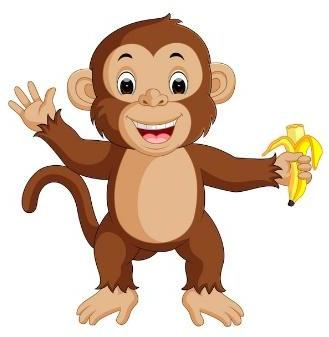
\includegraphics[width=.3\textwidth]{media/image218.jpg}
\end{figure}

QUAL FRASE REPRESENTA ESSA IMAGEM?

\begin{escolha}
\item O MACACO ESTÁ COMENDO A BANANA.

\item O MACACO JOGOU A BANANA NO CHÃO.

\item A BANANA DO MACACO CAIU.

\item A BANANA ESTÁ VERDE.
\end{escolha}

\pagebreak
\num{10} OBSERVE O ANIMAL QUE PEDRO GOSTA DE VISITAR NO ZOOLÓGICO.

\begin{figure}[htpb]
\centering
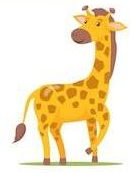
\includegraphics[width=.3\textwidth]{media/image219.jpg}
\end{figure}

ESCREVA O NOME DESSE ANIMAL.

\begin{escolha}
\item GIRAFA

\item IRAFA

\item GIRFA

\item A BANANA ESTÁ VERDE.
\end{escolha}

\num{11}

\begin{quote}
\begin{verse}
\textbf{A CASA FEIA}

O GATO FEZ UMA CASA\\
VEIO O RATO E FALOU:\\
- HUM! ... QUE CASA FEIA!\\
CASA BONITA TEM TELHADO,\\
LOGO, LOGO O GATO FEZ O TELHADO.\\
VEIO O PATO E FALOU:\\
- HUM QUE CASA FEIA!
\end{verse}
\end{quote}

\begin{quote}
\begin{verse}
CASA BONITA TEM VARANDA.\\
O GATO FEZ UMA VARANDA.\\
VEIO O BODE E FALOU:\\
-HUM... QUE CASA FEIA!\\
CASA BONITA É PINTADA.\\
E O GATO PINTOU A CASA.\\
MAS ELE FALOU:\\
-HUM... CASA BONITA TEM JARDIM.\\
VEIO O RATO, VEIO O PATO, VEIO O BODE DE NOVO.\\
-NOSSA! QUE CASA LINDA! - ELES DISSERAM.\\
E O GATO CONVIDOU TODOS PARA ENTRAR
\end{verse}

\fonte{Prefeitura de Bauru. A CASA FEIA. Disponível em: \emph{https://tinyurl.com/y5mzt3x8}. Acesso em: 14 abr. 2023.}
\end{quote}	

QUEM DISSE AO GATO QUE CASA BONITA TEM VARANDA? 

\begin{escolha}
\item RATO.

\item GATO.

\item PATO.

\item BODE.
\end{escolha}

\num{12}\enlargethispage{2\baselineskip}

\begin{quote}
\begin{verse}
\textbf{A BARATA}

A BARATA DIZ QUE TEM\\
SETE SAIAS DE FILÓ.\\
É MENTIRA DA BARATA\\
ELA TEM É UMA SÓ.
\end{verse}
\end{quote}

\begin{quote}
\begin{verse}
AH! AH! AH!\\
OH! OH! OH!\\
ELA TEM É UMA SÓ.\\
A BARATA DIZ QUE TEM\\
SETE SAIAS DE BALÃO.\\
É MENTIRA ELA NÃO TEM\\
NEM DINHEIRO PRO SABÃO.\\
AH! AH! AH!\\
OH! OH! OH!
\end{verse}

\fonte{ Domínio Público. ADIVINHAS, CANÇÕES, CANTIGAS DE RODA, PARLENDAS, POEMAS, QUADRINHAS E TRAVA-LÍNGUAS. Disponível em: \emph{http://www.dominiopublico.gov.br/download/texto/me000588.pdf}. Acesso em 14 abr. 2023.}
\end{quote}

QUAL É O ASSUNTO DESSE TEXTO?

\begin{escolha}
\item O DINHEIRO DA BARATA.

\item A MENTIRA DA BARATA.

\item O DESEJO DA BARATA.

\item A INVEJA DA BARATA.
\end{escolha}

\num{13} OBSERVE O TEXTO.

\begin{figure}[htpb]
\centering
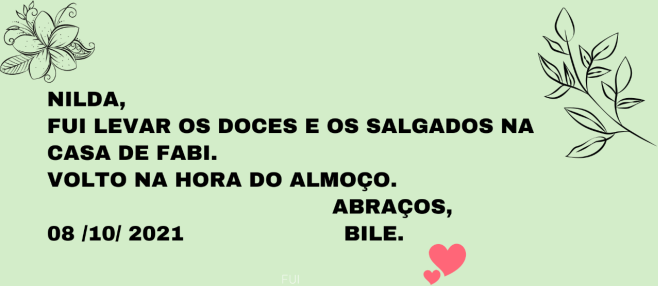
\includegraphics[width=.8\textwidth]{media/image220.png}
\end{figure}
%ELABORADO PELA AUTORA

\pagebreak
ESTE TEXTO SERVE PARA INDICAR

\begin{escolha}
\item DEIXAR UM RECADO.

\item DIVULGAR UM EVENTO.

\item ORGANIZAR AS TAREFAS.

\item ENSINAR A FAZER UMA COMIDA.
\end{escolha}

\num{14} LEIA O TEXTO:

\begin{quote}
\textbf{O LEÃO E O RATINHO}

UM LEÃO, CANSADO DE TANTO CAÇAR, DORMIA ESPICHADO À SOMBRA
DE UMA BOA ÁRVORE. VIERAM UNS RATINHOS PASSEAR EM CIMA DELE
E ELE ACORDOU.TODOS CONSEGUIRAM FUGIR, MENOS UM, QUE O LEÃO
PRENDEU EMBAIXO DA PATA. TANTO O RATINHO PEDIU E IMPLOROU
QUE O LEÃO DESISTIU DE ESMAGÁ-LO E DEIXOU QUE FOSSE EMBORA.
ALGUM TEMPO DEPOIS, O LEÃO FICOU PRESO NA REDE DE
UNS CAÇADORES. NÃO CONSEGUIA SE SOLTAR, E FAZIA A FLORESTA
INTEIRA TREMER COM SEUS URROS DE RAIVA.
NISSO, APARECEU O RATINHO. COM SEUS DENTES AFIADOS,
ROEU AS CORDAS E SOLTOU O LEÃO.

\fonte{Disponível
em: http://www.dominiopublico.gov.br/download/texto/me001614.pdf Acesso em: 
20 fev. 2023.}
\end{quote}

O RATINHO AJUDOU O LEÃO PORQUE ELE

\begin{escolha}
\item ERA MUITO BONZINHO E GENTIL.

\item ERA MUITO VALENTE E RAIVOSO.

\item TINHA-O ESMAGADO UM DIA.

\item TINHA-O AJUDADO NO PASSADO.
\end{escolha}

\pagebreak
\num{15} LEIA O DIÁLOGO E OBSERVE A IMAGEM.

\begin{figure}[htpb]
\centering
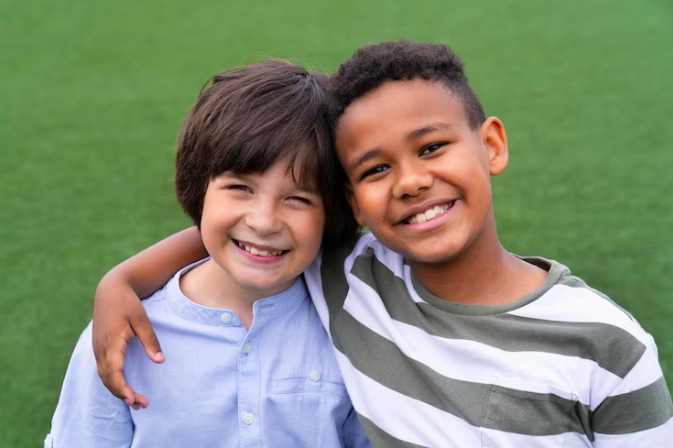
\includegraphics[width=\textwidth]{media/image220b.png}
\end{figure}

\begin{quote}
— CHEGOU DE VIAGEM, LUCAS?

— ISSO MESMO, BETO. CHEGUEI ONTEM À NOITE.

— ENTÃO HOJE NÃO TEREI DE BRINCAR SOZINHO?

— NÃO MESMO!

— EBA!
\end{quote}

BETO FICOU FELIZ PORQUE

\begin{escolha}
\item TEM SEU CACHORRO.

\item GANHOU UM CACHORRO.

\item GANHOU UM CARRINHO.

\item TEM UM AMIGO PRA BRINCAR.
\end{escolha}

\blankpage

% \vspace*{-4.2cm}
% \hspace*{-4cm}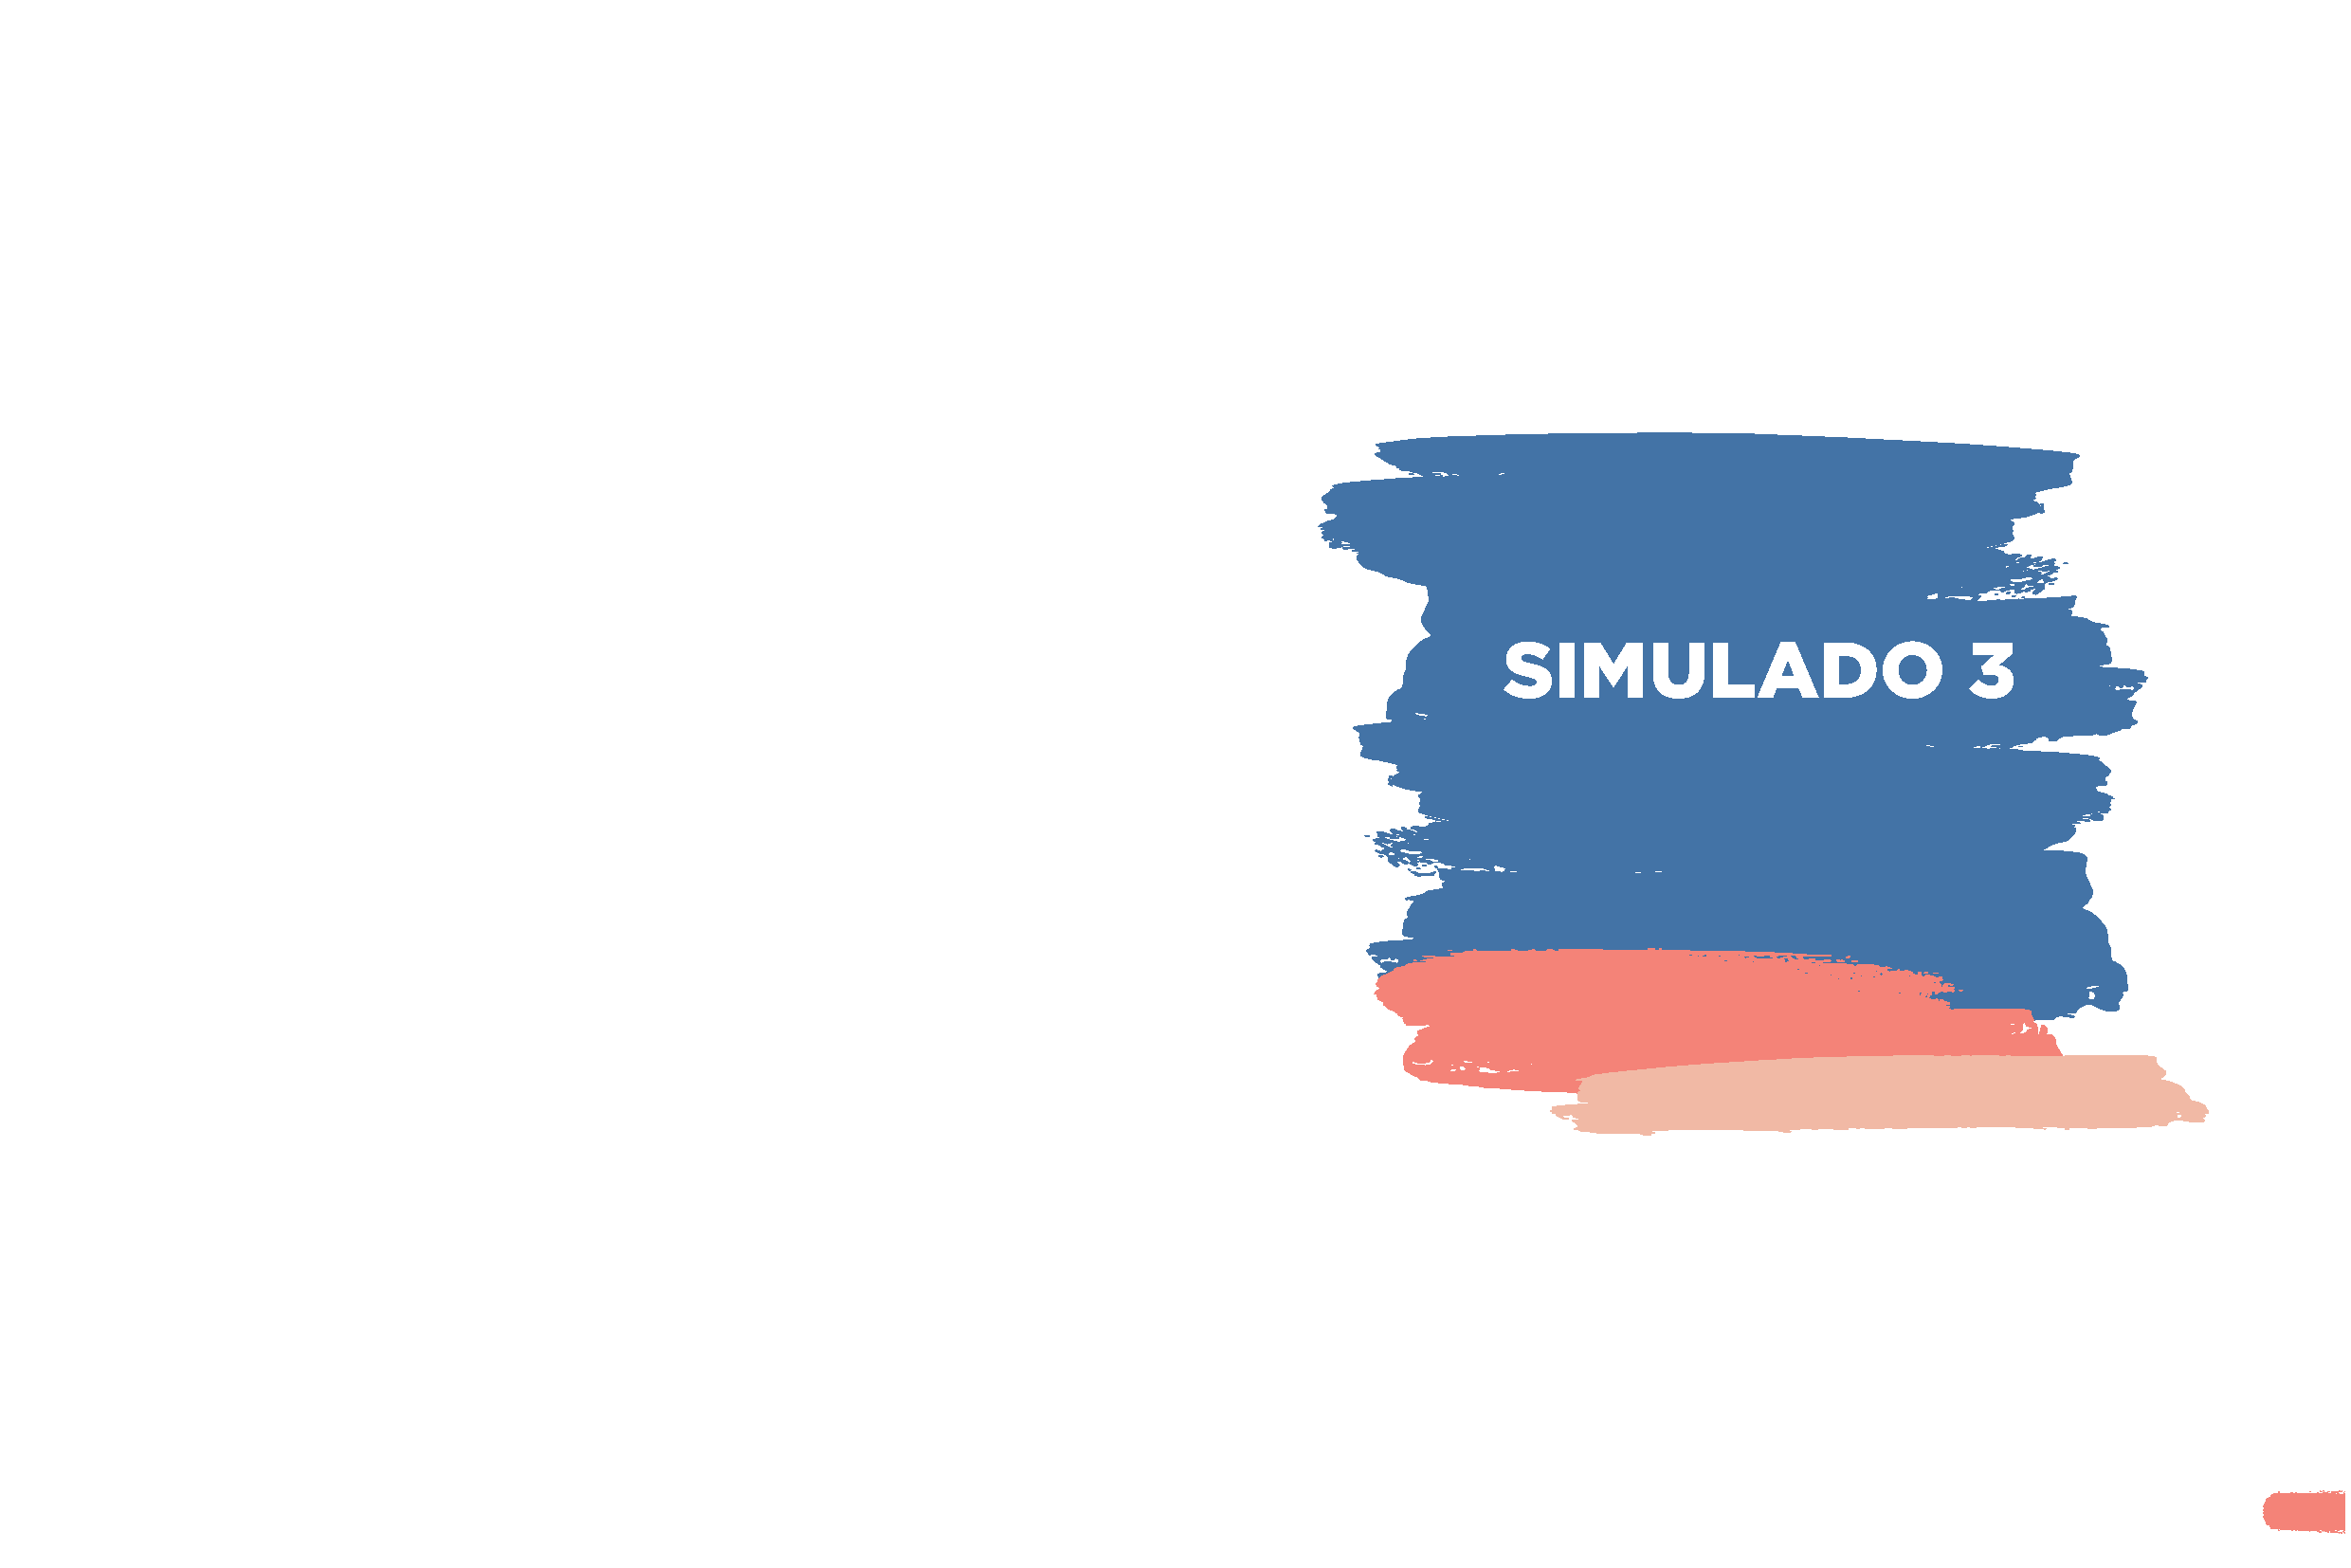
\includegraphics[scale=1]{../watermarks/3simulado5ano.pdf}

\addcontentsline{toc}{chapter}{SIMULADO 3}
\markboth{Simulado 3}{}

\pagebreak

\num{1} IZABEL VAI ESCOLHER UMA PLACA PARA ESCREVER O SEU NOME EM UM JOGO.

\begin{escolha}
\item 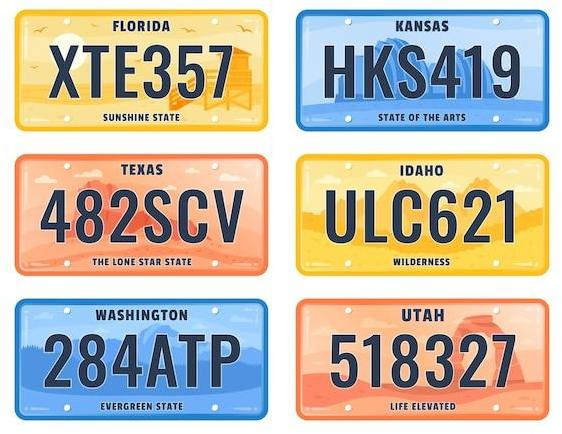
\includegraphics[width=2.32569in,height=1.18472in]{media/image222.jpg}

\item 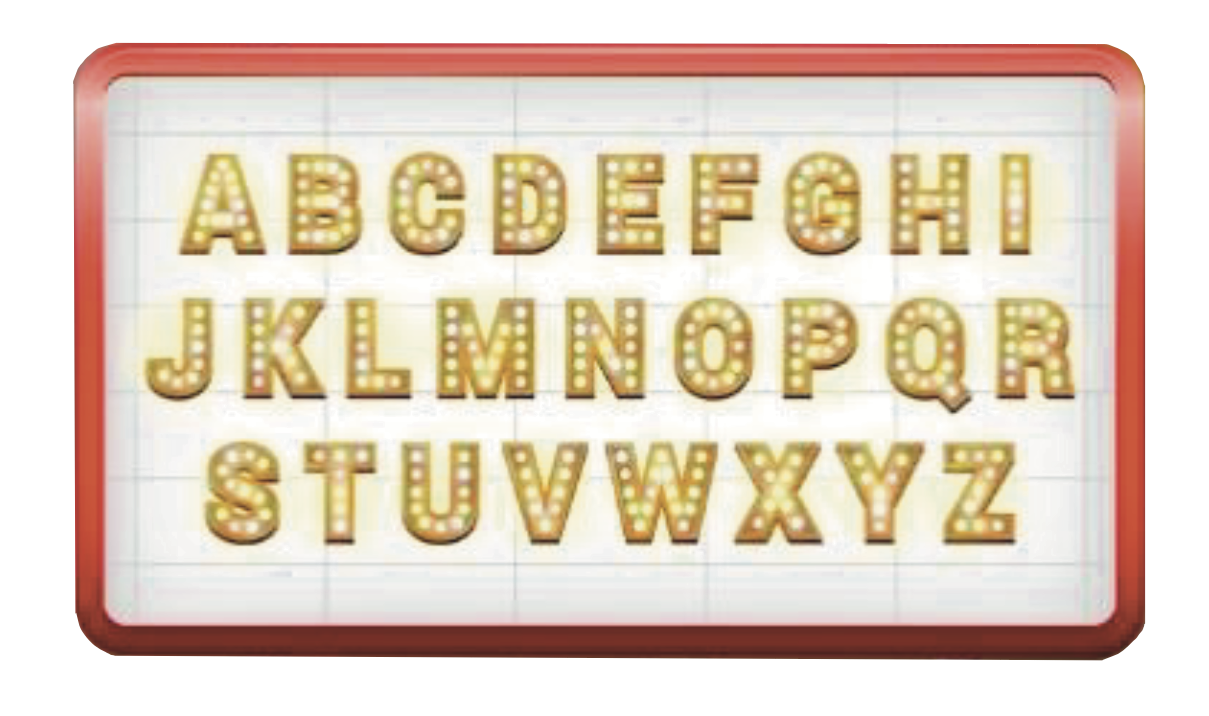
\includegraphics[width=2.03125in,height=1.17361in]{media/image223.png}

\item 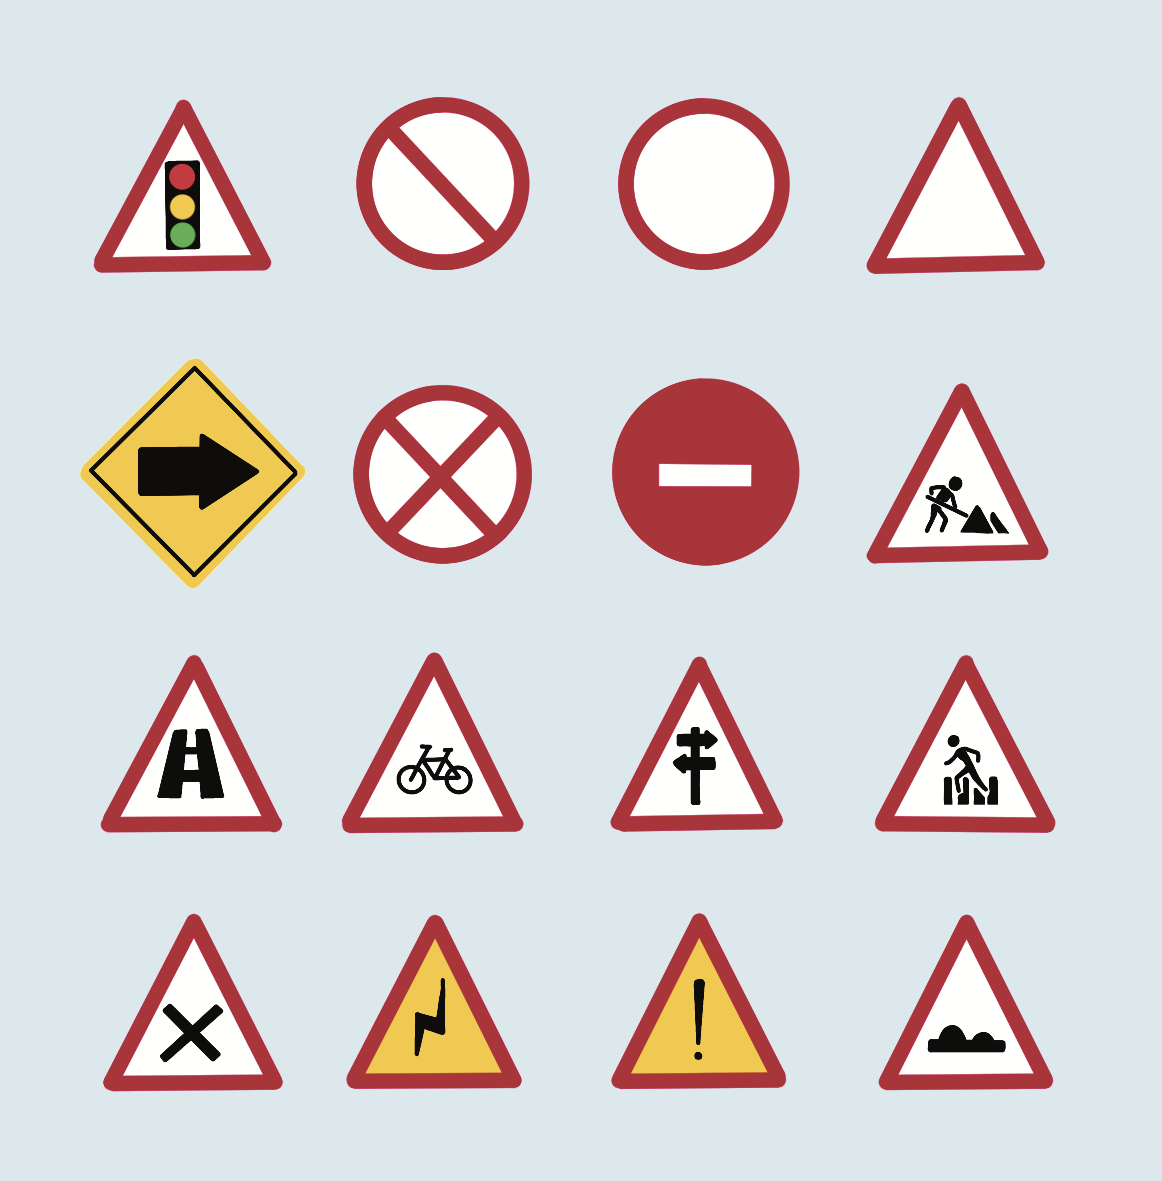
\includegraphics[width=2.20764in,height=1.07569in]{media/image224.png}

\item 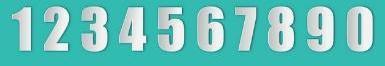
\includegraphics[width=1.75000in,height=0.54792in]{media/image225.jpg}
\end{escolha}

\num{2} VEJA O NOME QUE MIGUEL ESCOLHEU PARA SEU CACHORRO. 

\begin{figure}[htpb]
\centering
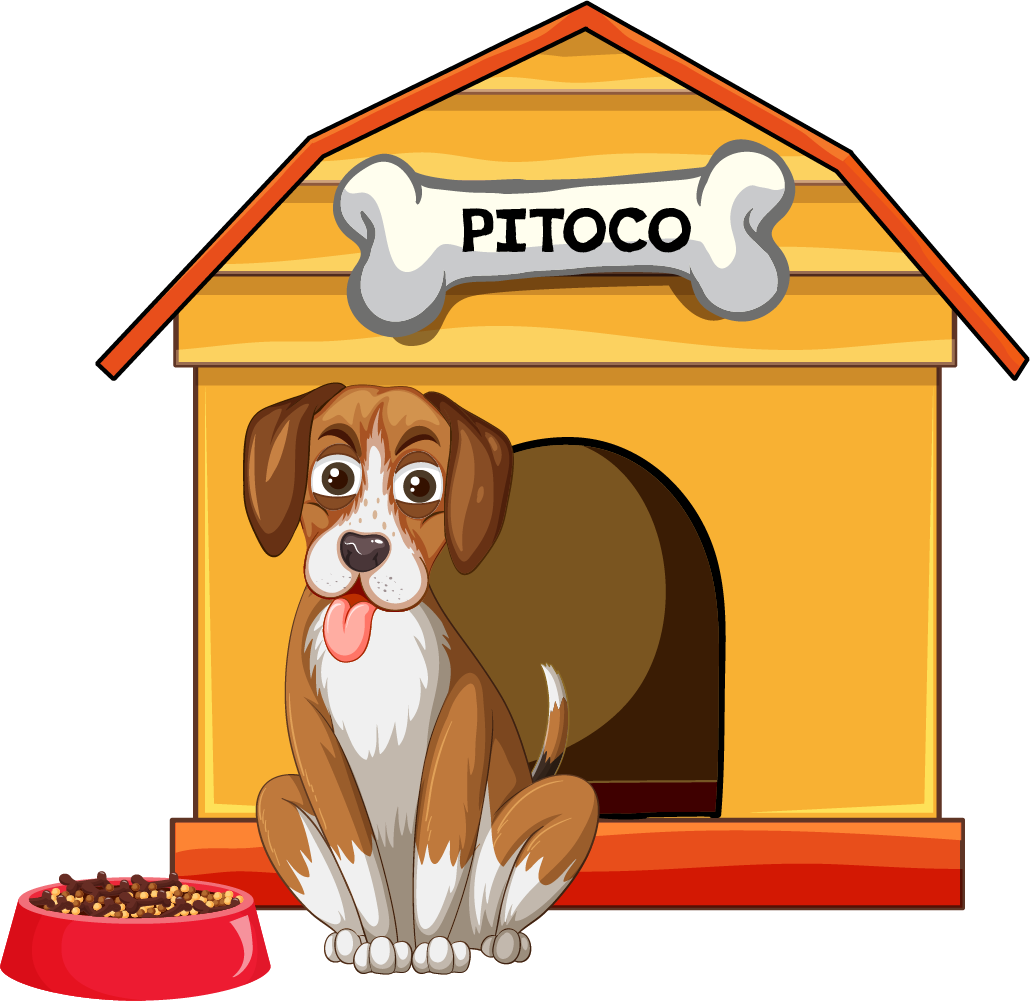
\includegraphics[width=.5\textwidth]{media/image226.png}
\end{figure}

QUAL PALAVRA TEM A MESMA QUANTIDADE DE VOGAIS DO NOME DO CACHORRO?

\begin{escolha}
\item FADA.

\item CAVALO.

\item TELEVISÃO.

\item GELATINA.
\end{escolha}

\num{3} OBSERVE O DESENHO QUE BIANCA COLORIU.

\begin{figure}[htpb]
\centering
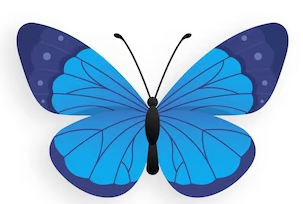
\includegraphics[width=.5\textwidth]{media/image227.png}
\end{figure}


A PALAVRA QUE TERMINA COM A MESMA SÍLABA DO NOME DO ANIMAL DESENHADO É

\begin{escolha}
\item BATATA.

\item TAPETE.

\item BONECA.

\item GILETE.
\end{escolha}

\pagebreak
\num{4} VEJA A PALAVRA NOVA QUE JOANA ESCREVEU NO SEU CADERNO.

\begin{figure}[htpb]
\centering
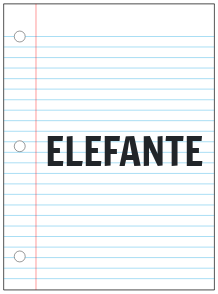
\includegraphics[width=.25\textwidth]{media/image230.png}
\end{figure}

AS LETRAS QUE FORMAM O SOM FINAL DA PALAVRA QUE ELA ESCREVEU SÃO

\begin{escolha}
\item E+E.

\item L+E

\item F+A

\item T+E
\end{escolha}

\num{5} VEJA A PALAVRA QUE UMA MENINA ESCREVEU NA LOUSA.

\begin{myquote}
CAVALO
\end{myquote}

A SÍLABA MEDIAL DESSA PALAVRA É

\begin{escolha}
\item CA.

\item VA.

\item LO

\item OL.
\end{escolha}

\pagebreak
\num{6} LEIA.

\begin{quote}
\begin{verse}
CARANGUEJO PEIXE É.\\
CARANGUEJO NÃO É PEIXE,\\
CARANGUEJO PEIXE É,\\
CARANGUEJO SÓ É PEIXE\\
NA VAZANTE DA MARÉ.
\end{verse}

\fonte{Domínio Público. ADIVINHAS, CANÇÕES, CANTIGAS DE RODA, PARLENDAS, POEMAS, QUADRINHAS E TRAVA-LÍNGUAS. Disponível em: \emph{https://bit.ly/2svTEzT}. Acesso em 14 abr. 2023. }
\end{quote}

A ÚLTIMA PALAVRA DO TEXTO É

\begin{escolha}
\item CARANGUEJO.

\item VAZANTE.

\item PEIXE.

\item MARÉ.
\end{escolha}

\num{7} LEIA A PALAVRA.

\begin{myquote}
\textbf{BOLA}
\end{myquote}

A PALAVRA EM QUE NÃO APARECE NENHUMA SÍLABA PERTENCENTE À PALAVRA QUE VOCÊ LEU É 

\begin{escolha}
\item BOLO.

\item LATA.

\item LOBO.

\item FADA.
\end{escolha}

\pagebreak
\num{8} VEJA O PRESENTE QUE TALIA DEU PARA SUA AMIGA NO SEU ANIVERSÁRIO.

\begin{figure}[htpb]
\centering
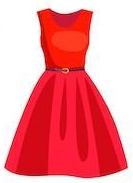
\includegraphics[width=.25\textwidth]{media/image232.jpg}
\end{figure}

ESCREVA O NOME DO PRESENTE QUE ELA GANHOU.

\begin{escolha}
\item VESTIDO.

\item VETIDO.

\item ETIDO.

\item VETDO.
\end{escolha}

\num{9} OBSERVE ESSA IMAGEM.

\begin{figure}[htpb]
\centering
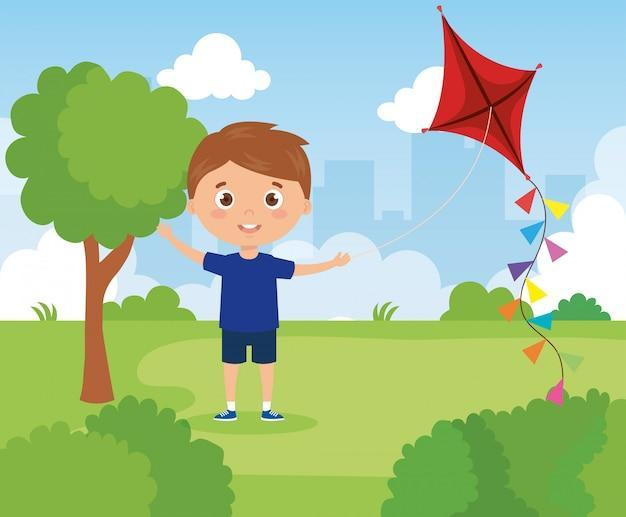
\includegraphics[width=.55\textwidth]{media/image233.jpg}
\end{figure}

\pagebreak
A FRASE QUE REPRESENTA A IMAGEM É

\begin{escolha}
\item O MENINO SOBE NA ÁRVORE.

\item O MENINO BRINCA COM A PIPA.

\item O MENINO TOMA BANHO NO RIO.

\item O MENINO SE ESCONDE ATRÁS DO ARBUSTO.
\end{escolha}

\num{10} VEJA O ANIMAL PREFERIDO DE BRUNO.

\begin{figure}[htpb]
\centering
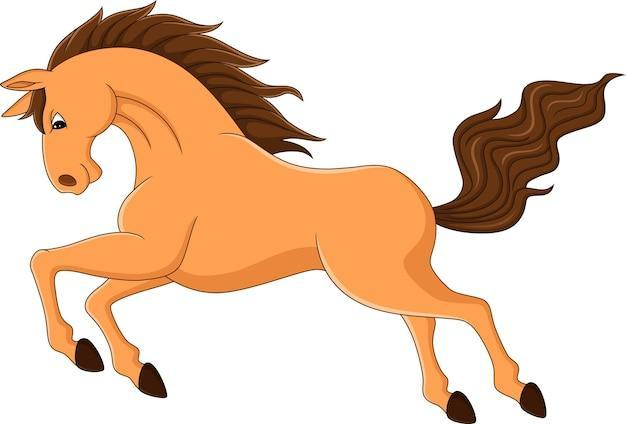
\includegraphics[width=.3\textwidth]{media/image234.jpg}
\end{figure}


O NOME CORRETO DESSE ANIMAL É

\begin{escolha}
\item VALO

\item KAVA

\item CAVALO

\item VALOCA
\end{escolha}

\num{11} OBSERVE O MÓVEL QUE CARLA COMPROU PARA SEU QUARTO.

\begin{figure}[htpb]
\centering
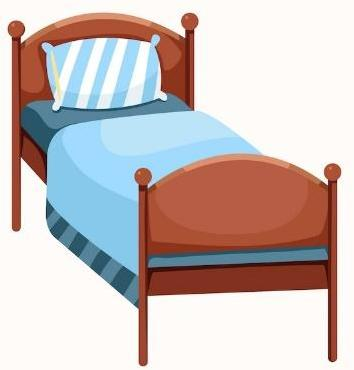
\includegraphics[width=.2\textwidth]{media/image235.jpg}
\end{figure}

\pagebreak

A PALAVRA QUE COMEÇA COM O MESMO SOM FINAL DO NOME DO MÓVEL DE CARLA É 

\begin{escolha}
\item CANELA.

\item BONECA.

\item SACADA.

\item MACACO.
\end{escolha}

\num{12} LEIA

\begin{quote}
\begin{verse}
SAPO CURURU\\
DA BEIRA DO RIO\\
QUANDO O SAPO GRITA\\
OH! MANINHA\\
É PORQUE TEM FRIO.
\end{verse}

\fonte{Domínio Público. ADIVINHAS, CANÇÕES, CANTIGAS DE RODA, PARLENDAS, POEMAS, QUADRINHAS E TRAVA-LÍNGUAS. Disponível em: \emph{http://www.dominiopublico.gov.br/download/texto/me000588.pdf}. Acesso em 14 abr. 2023.}
\end{quote}

POR QUE O SAPO GRITOU?

\begin{escolha}
\item PORQUE ESTÁ ASSUSTADO. 

\item PORQUE TEM FRIO.

\item PORQUE ESTÁ BRINCANDO.

\item PORQUE QUER ASSUSTAR SEUS AMIGOS.
\end{escolha}

\pagebreak
\num{13} LEIA A LISTA.

\begin{quote}
\begin{enumerate}
\item ARROZ

\item FEIJÃO

\item MACARRÃO

\item ÓLEO

\item BISCOITO.

\item EXTRATO

\item FARINHA

\item LEITE
\end{enumerate}
\end{quote}

ESSE TEXTO SERVE PARA

\begin{escolha}
\item ORGANIZAR TAREFAS.

\item ENSINAR A FAZER UM PRATO.

\item INDICAR OS PRODUTOS.

\item DIVULGAR UM EVENTO.
\end{escolha}

\num{14} LEIA O TEXTO. \enlargethispage{2\baselineskip}

\begin{quote}
\begin{verse}
\textbf{TEREZINHA DE JESUS}

TEREZINHA DE JESUS\\
DE UMA QUEDA FOI AO CHÃO\\
ACUDIRAM TRÊS CAVALHEIROS\\
TODOS TRÊS, CHAPÉU NA MÃO.
\end{verse}
\end{quote}

\begin{quote}
\begin{verse}
O PRIMEIRO, FOI SEU PAI\\
O SEGUNDO, SEU IRMÃO\\
O TERCEIRO FOI AQUELE\\
A QUE TERESA DEU A MÃO.

\fonte{Domínio Público. ADIVINHAS, CANÇÕES, CANTIGAS DE RODA, PARLENDAS, POEMAS, QUADRINHAS E TRAVA-LÍNGUAS. Disponível em: \emph{https://bit.ly/2svTEzT}. Acesso em 14 abr. 2023. }
\end{verse}
\end{quote}

DE QUE O TEXTO FALA?

\begin{escolha}
\item DO PAI DA TEREZINHA.

\item DA MÃO DA TEREZINHA.

\item DO IRMÃO DA TEREZINHA.

\item DA QUEDA DE TEREZINHA.
\end{escolha}

\num{15} \enlargethispage{2\baselineskip}

\begin{quote}
\textbf{A RAPOSA E O CORVO}

O CORVO CONSEGUIU ARRANJAR UM PEDAÇO DE QUEIJO, EM ALGUM
LUGAR. SAIU VOANDO, COM O QUEIJO NO BICO, ATÉ POUSAR NUMA
ÁRVORE.

QUANDO VIU O QUEIJO, A RAPOSA RESOLVEU SE APODERAR
DELE. CHEGOU AO PÉ DA ÁRVORE E COMEÇOU A BAJULAR O CORVO:

--- Ó SENHOR CORVO! O SENHOR É CERTAMENTE O MAIS BELO
DOS ANIMAIS! SE SOUBER CANTAR TÃO BEM QUANTO A SUA PLUMAGEM
É LINDA, NÃO HAVERÁ AVE QUE POSSA SE COMPARAR AO SENHOR.

\fonte{Disponível em:
\emph{http://www.dominiopublico.gov.br/download/texto/me001614.pdf}.
Acesso em: 20 fev. 2023.}
\end{quote}

A RAPOSA QUERIA QUE O CORVO CANTASSE PARA

\begin{escolha}
\item ALEGRAR A FLORESTA.

\item MOSTRAR SEU TALENTO.

\item GANHAR ELOGIOS.

\item PEGAR O QUEIJO..
\end{escolha}

\num{16} LEIA A TIRINHA.

\begin{figure}[htpb]
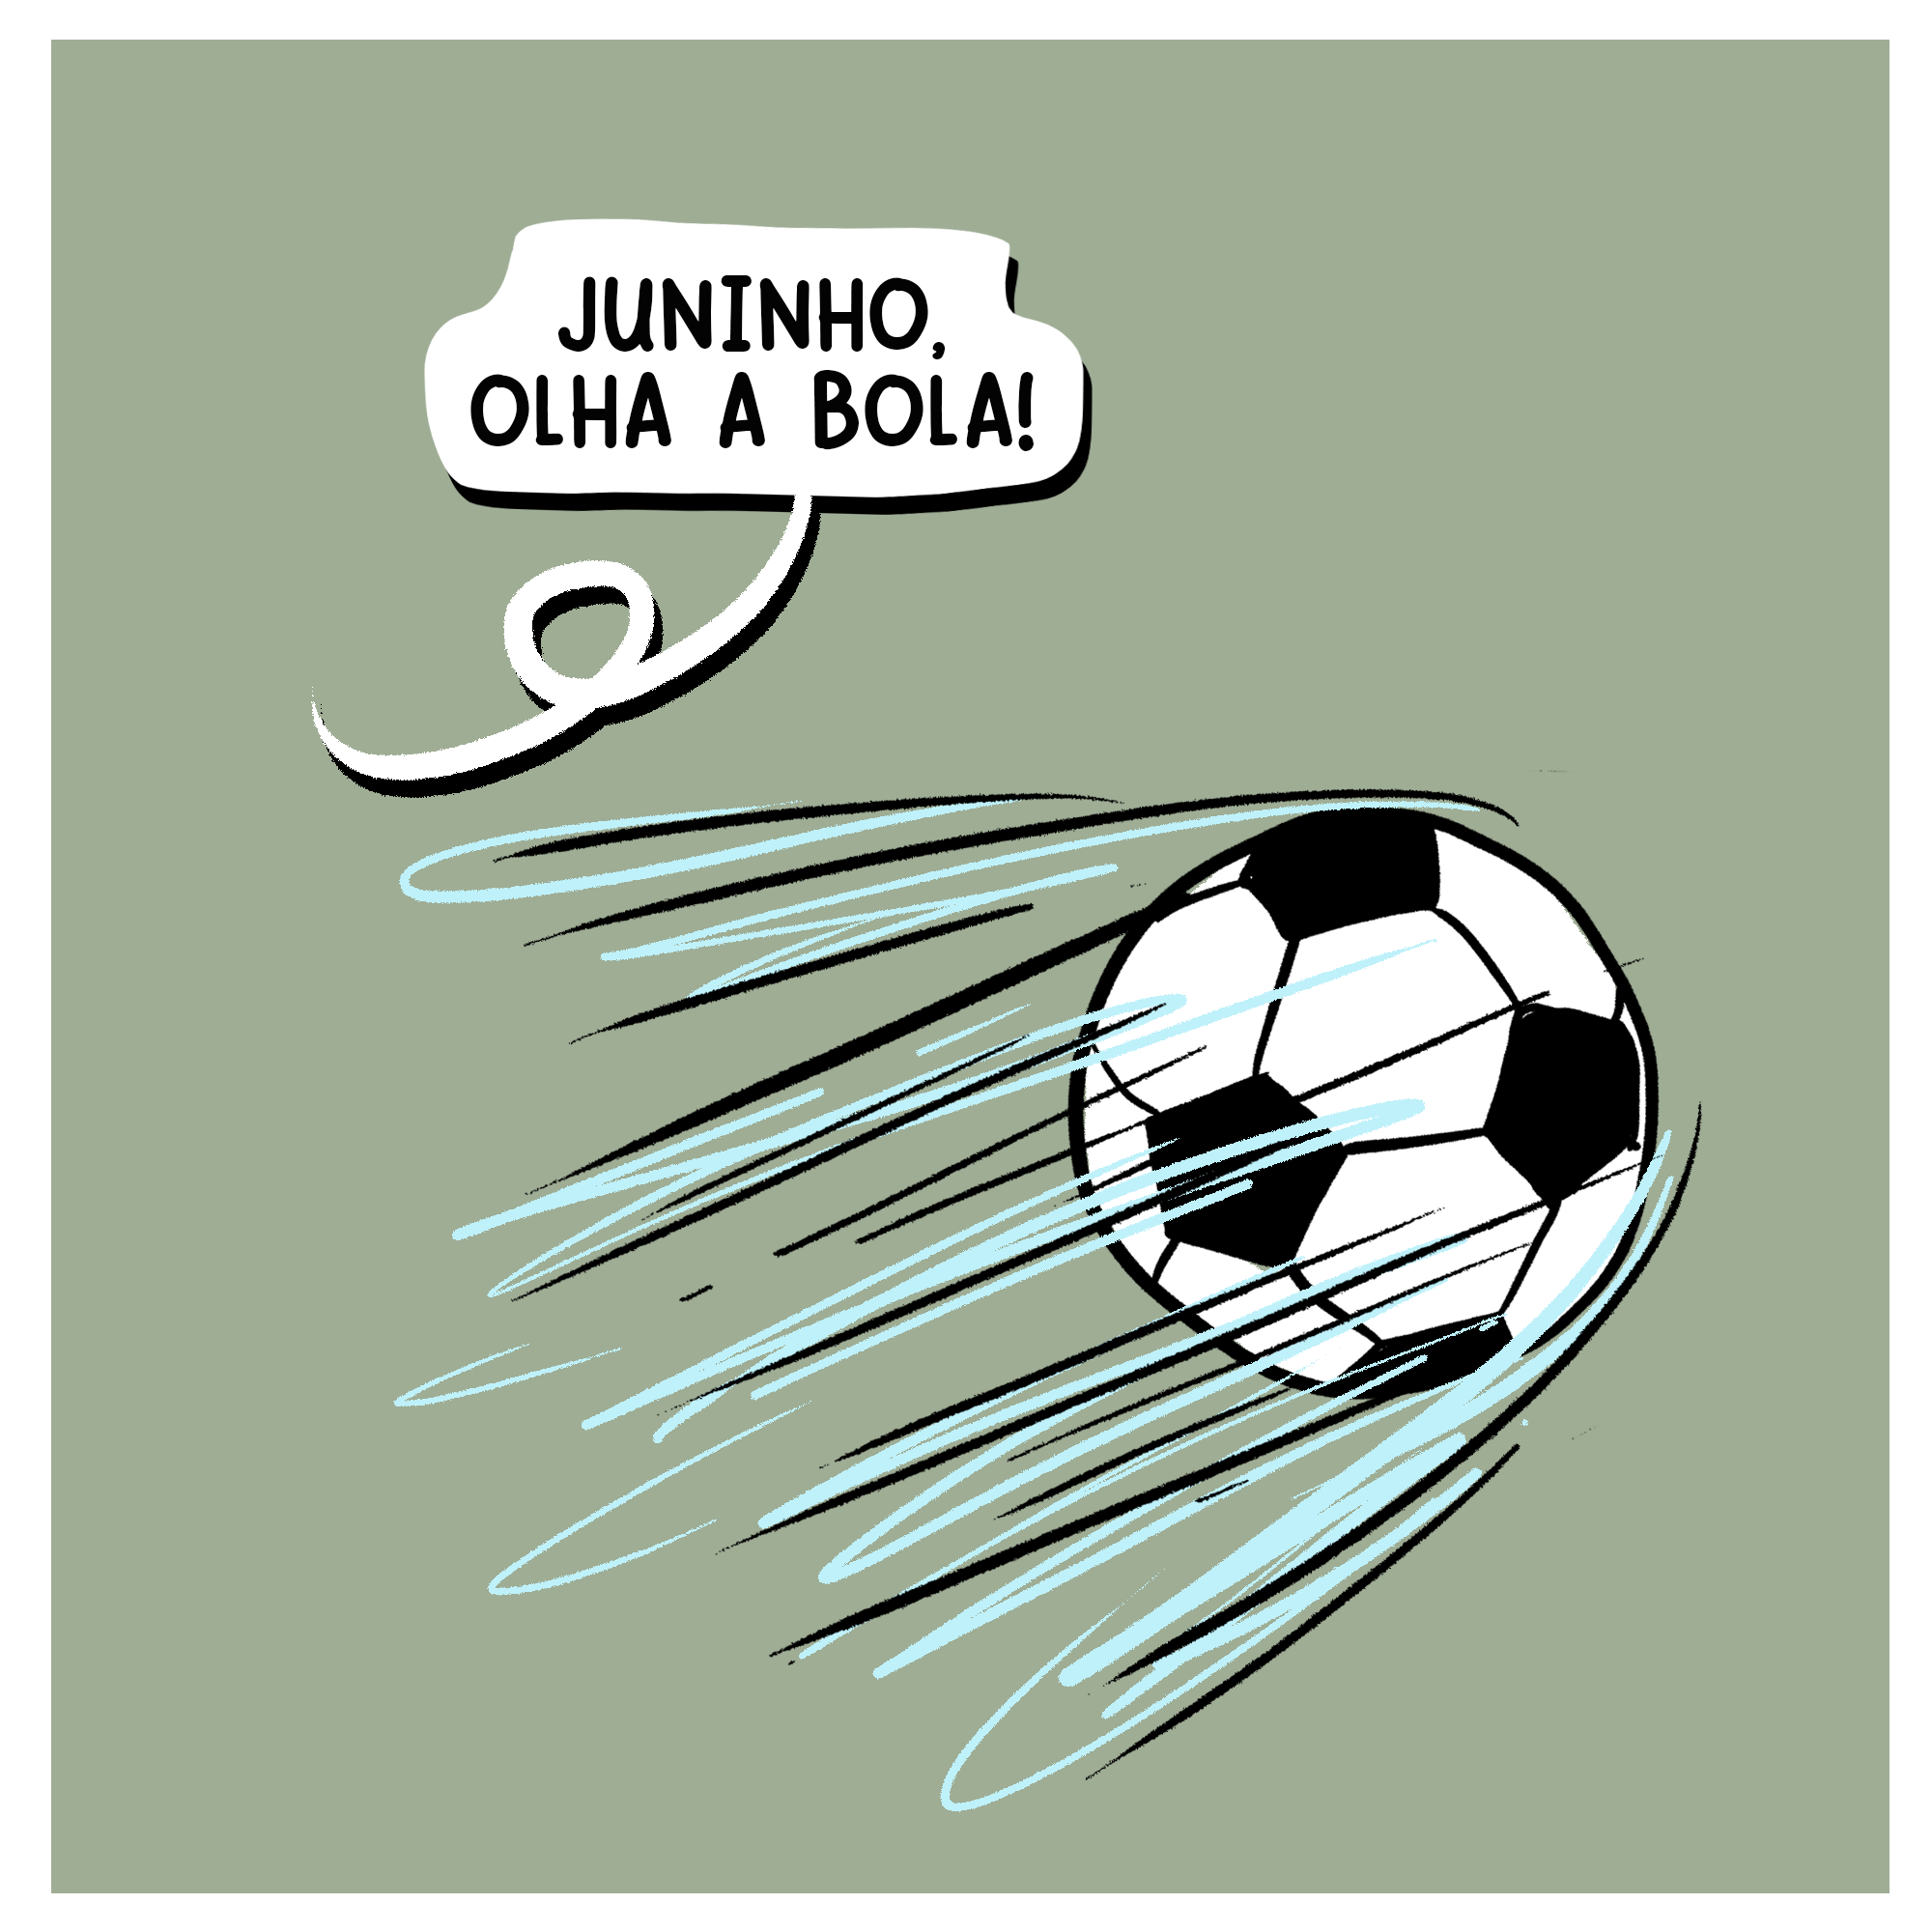
\includegraphics[width=1.88542in,height=1.88542in]{media/image236.png}
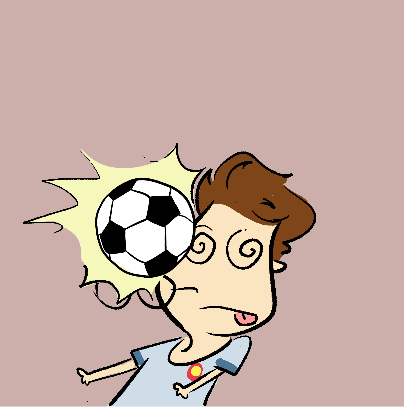
\includegraphics[width=1.92708in,height=1.92708in]{media/image237.png}
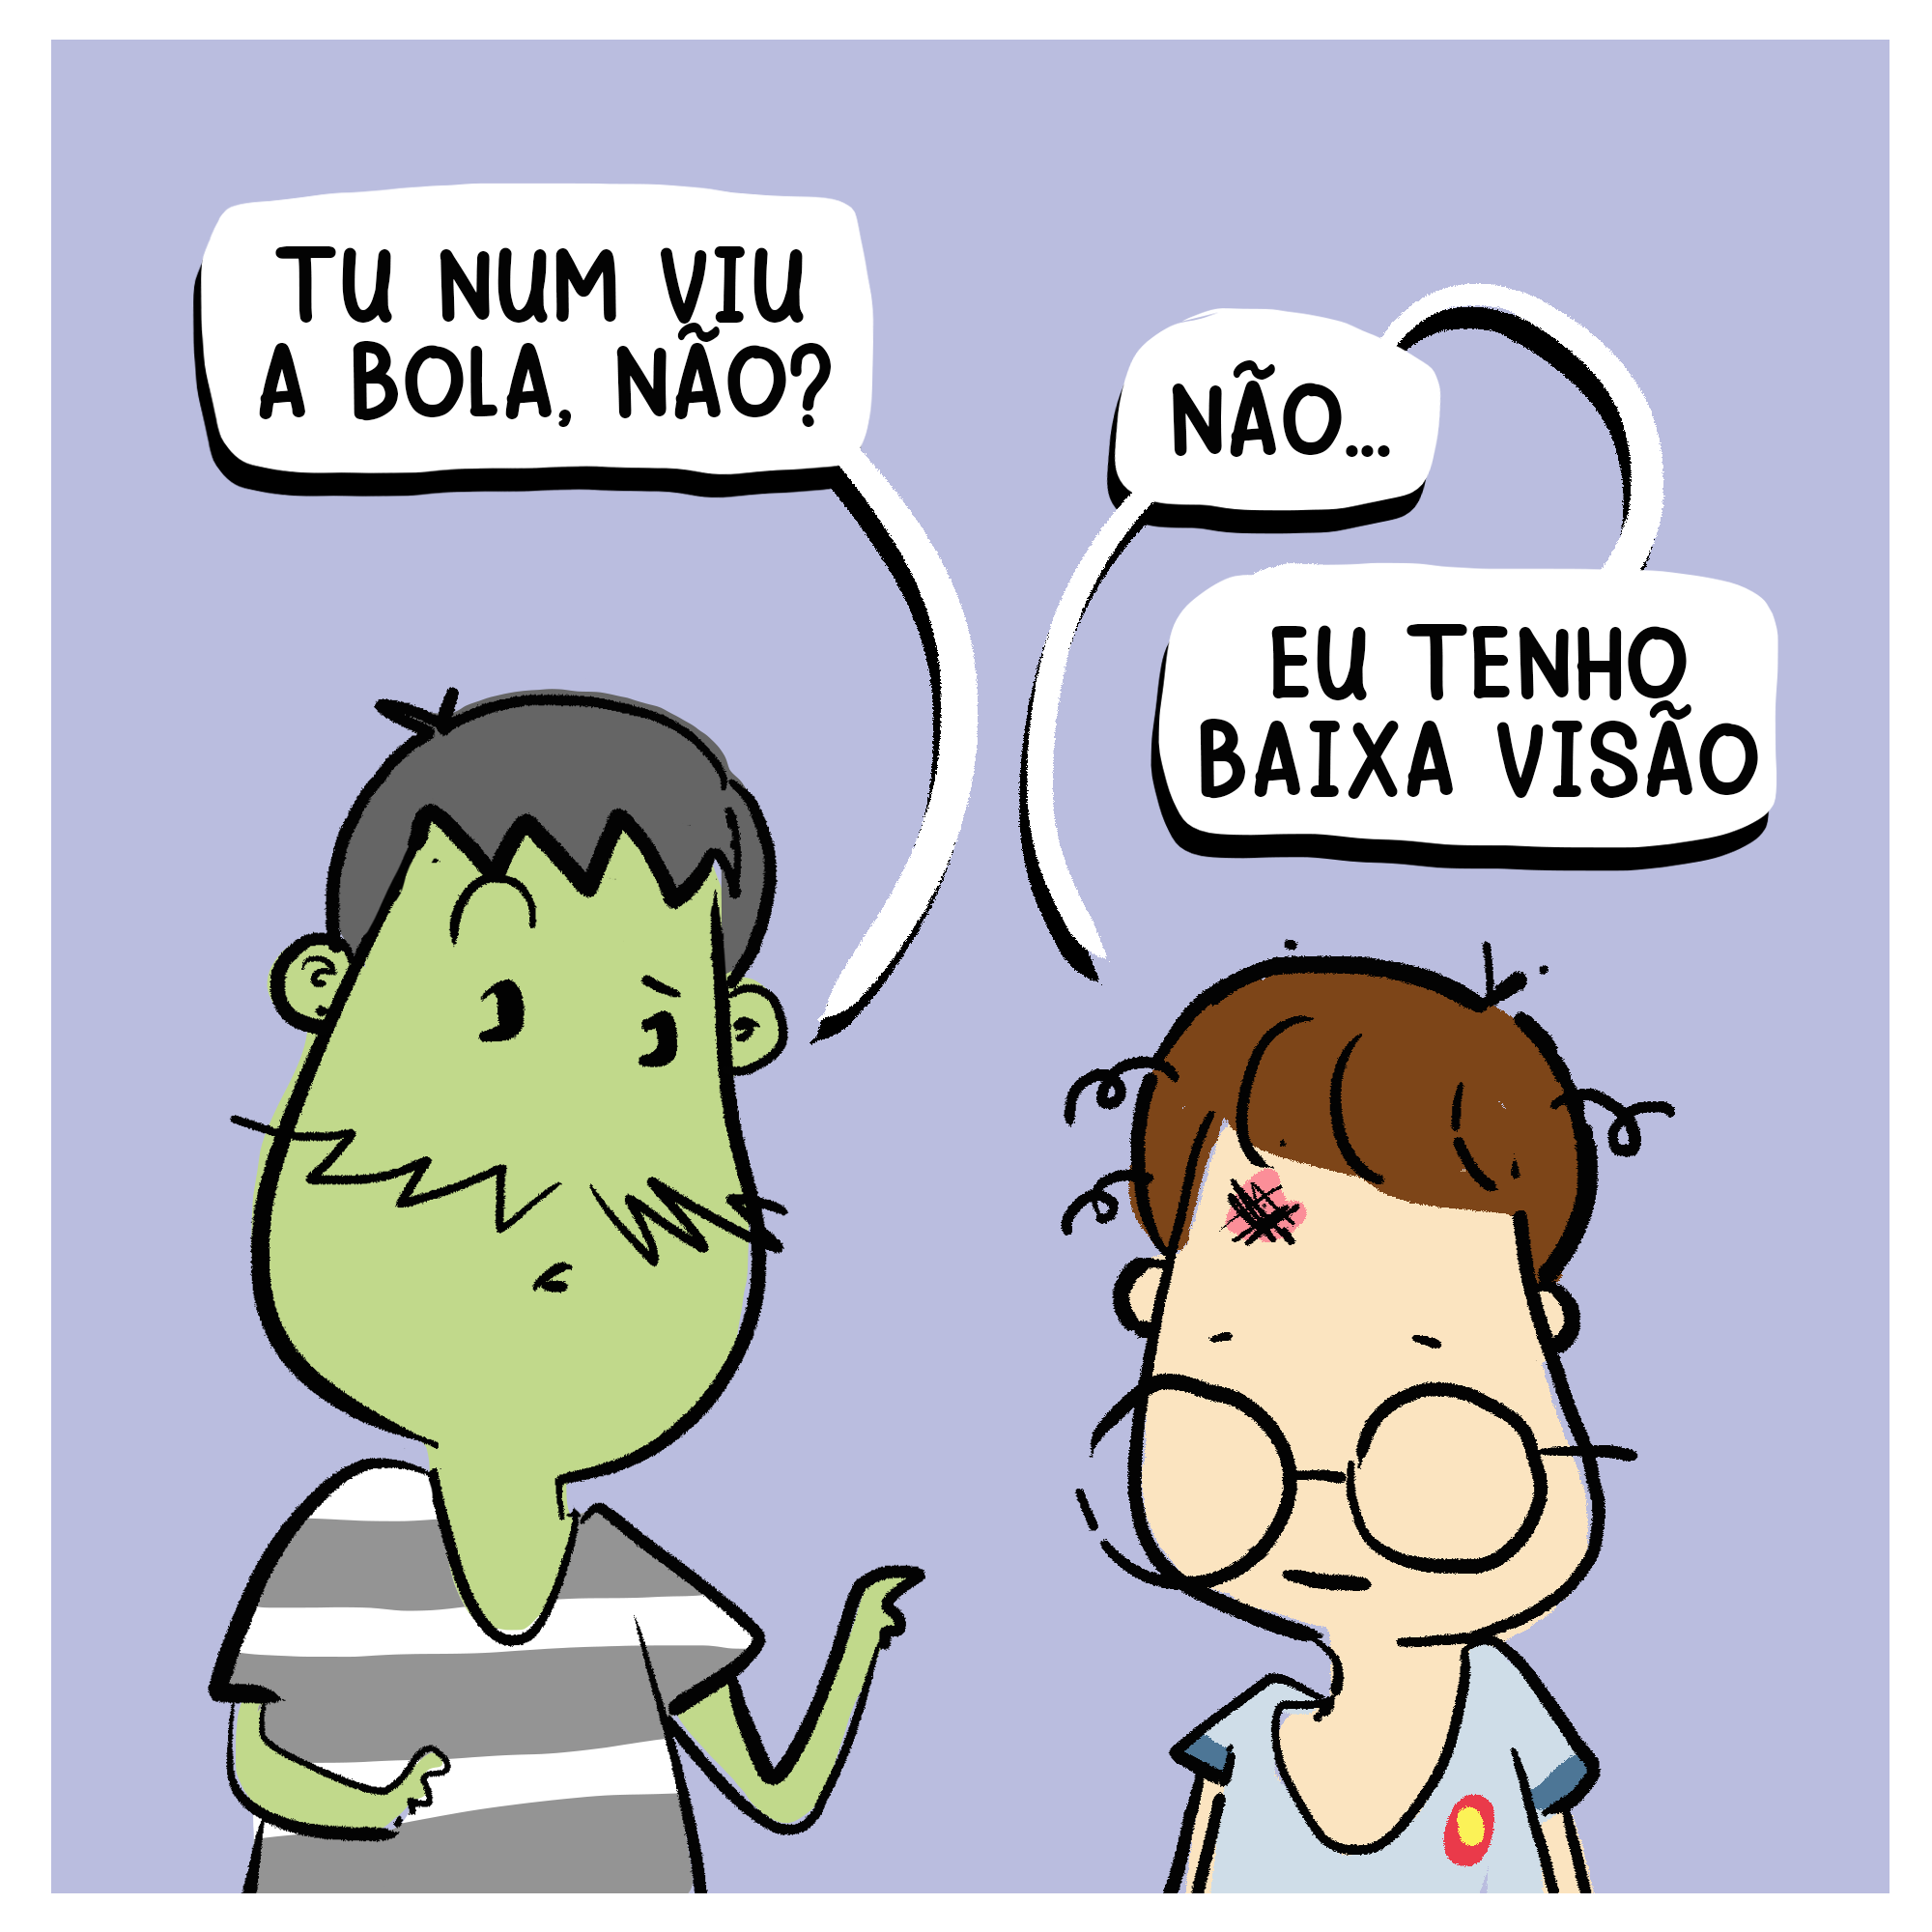
\includegraphics[width=1.90625in,height=1.90625in]{media/image238.png}
\end{figure}

%Disponível em https://lizeseusamigos.org.br/tirinhas/tirinhas-tres. Acesso 20 Fev 2023.

A BOLA ACERTOU JUNINHO NO SEGUNDO QUADRINHO PORQUE ELE

\begin{escolha}
\item É MUITO DISTRAÍDO.

\item TENTOU PEGAR A BOLA. 

\item ESTAVA JOGANDO COMO GOLEIRO.

\item TEM DIFICULDADE DE ENXERGAR.
\end{escolha}

\blankpage

% \vspace*{-4.2cm}
% \hspace*{-4cm}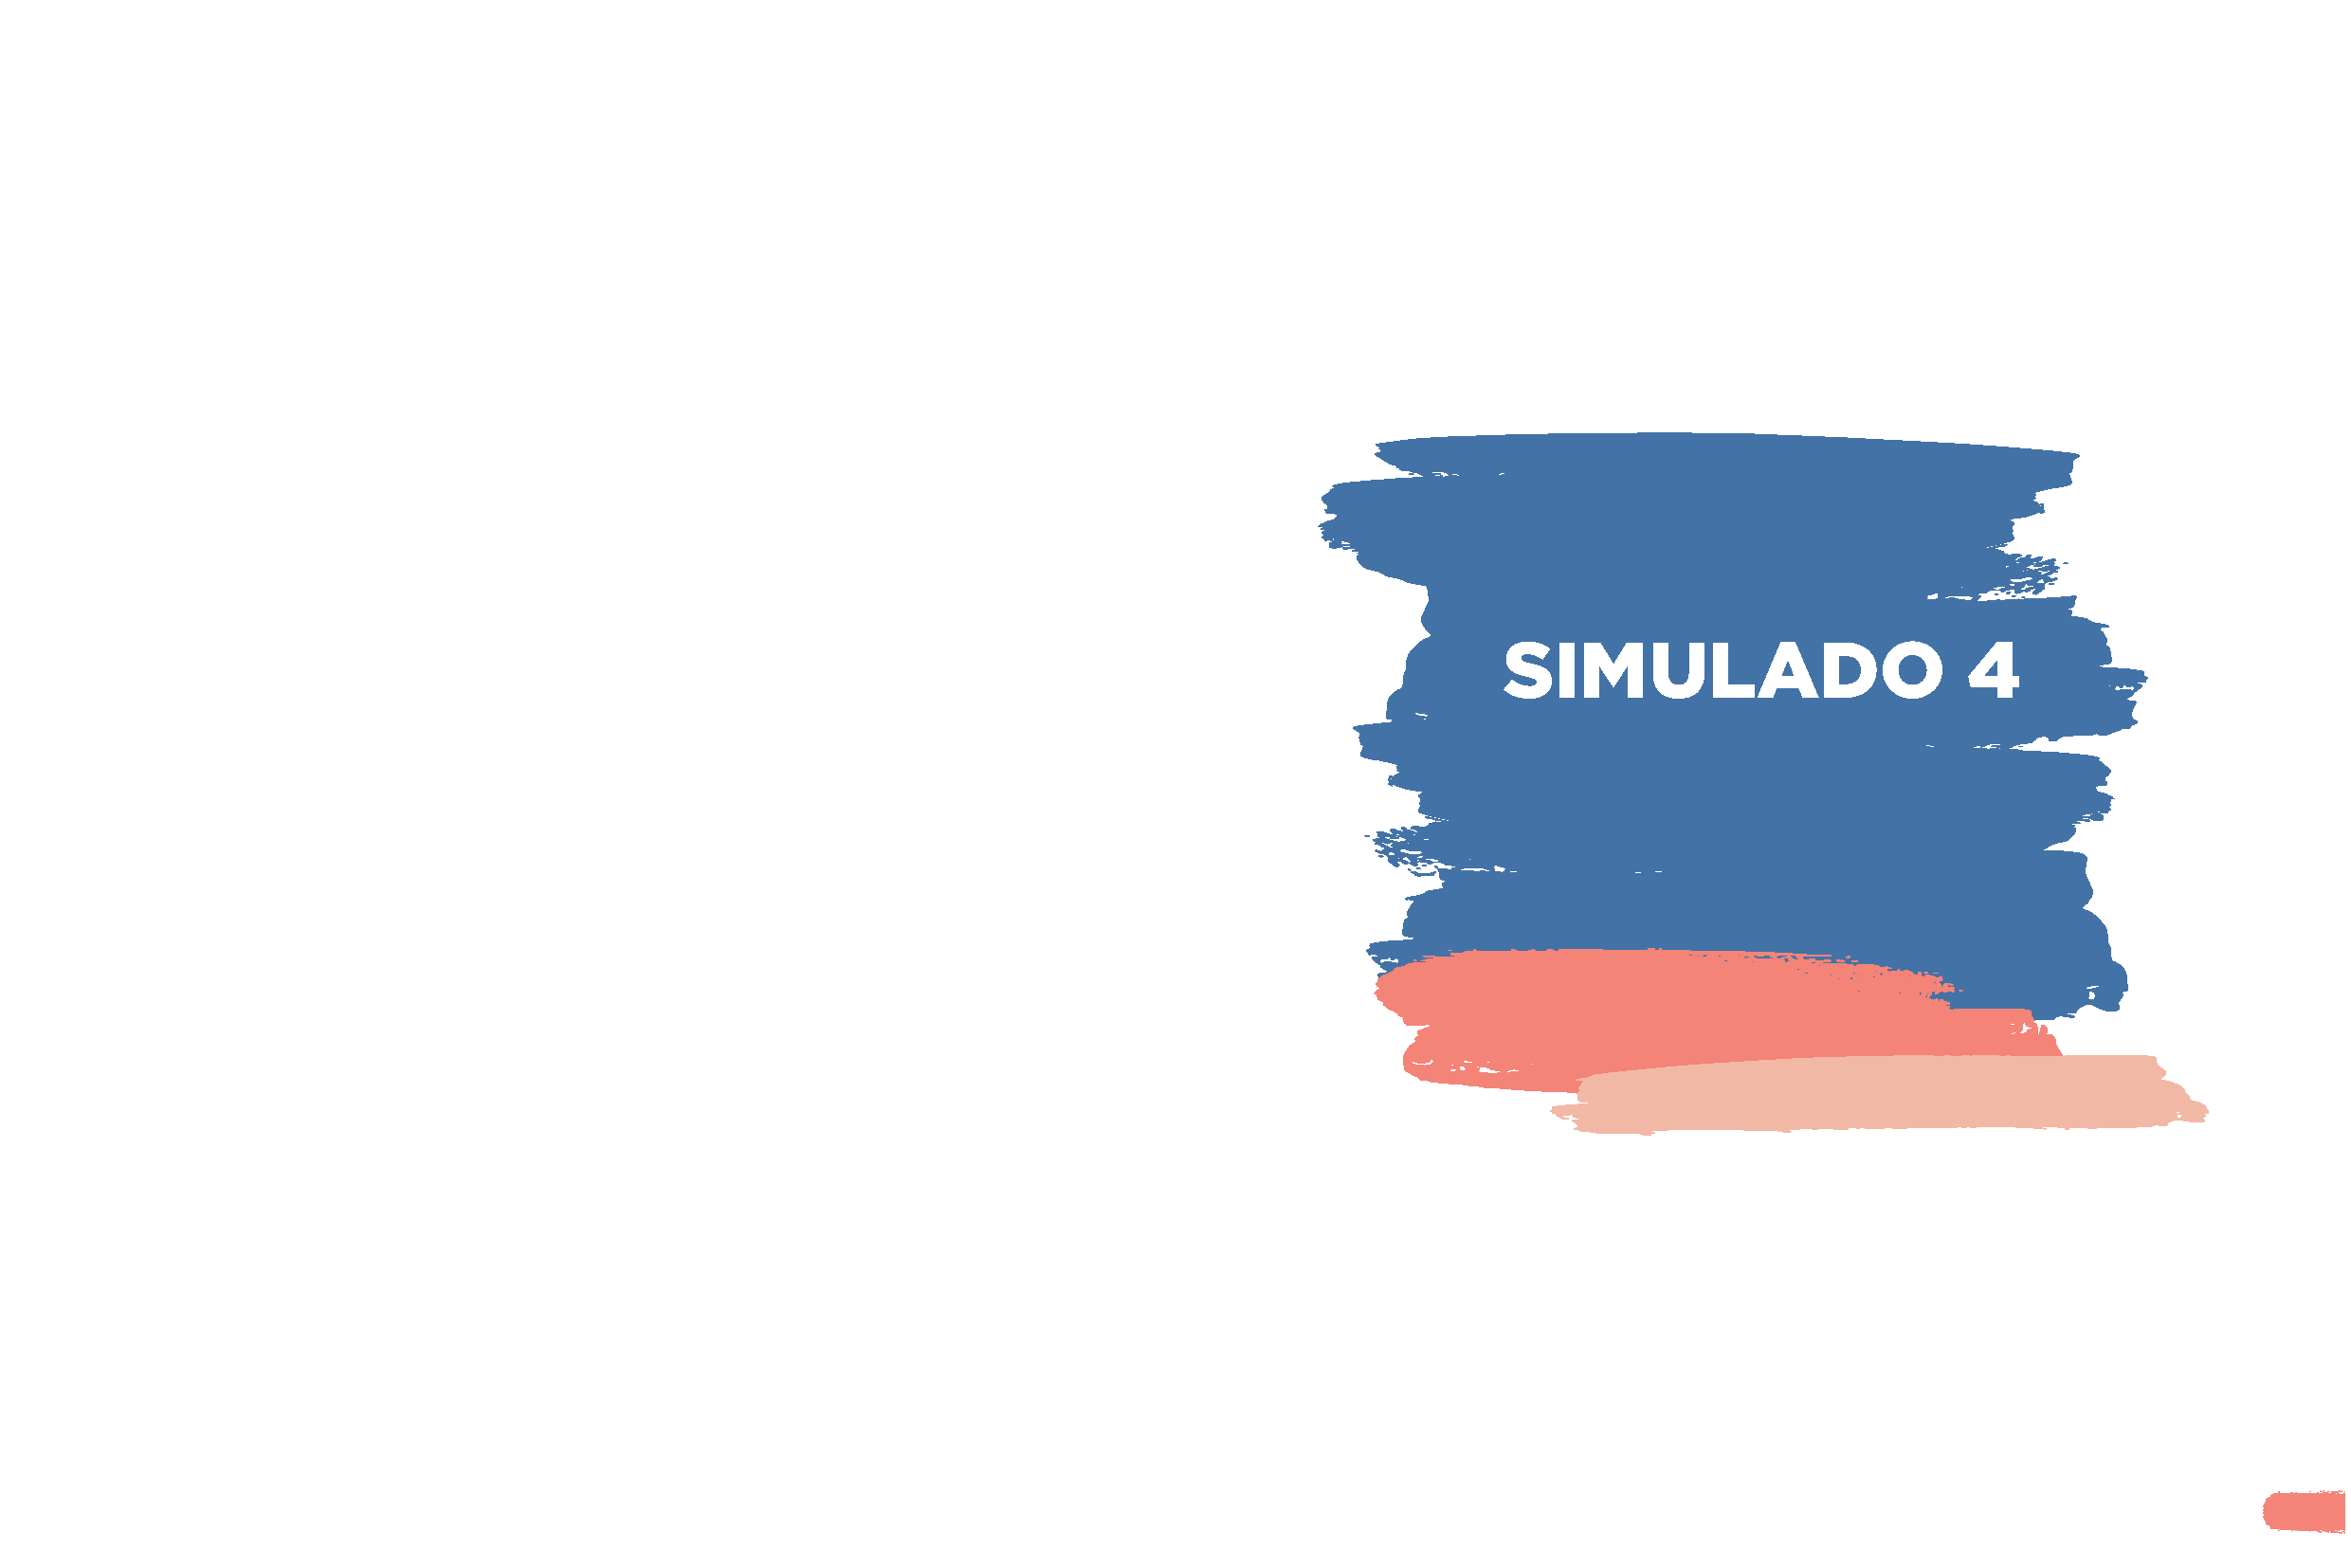
\includegraphics[scale=1]{../watermarks/4simulado5ano.pdf}

\addcontentsline{toc}{chapter}{SIMULADO 4}
\markboth{Simulado 4}{}

\pagebreak

\num{1} BIA QUER MOSTRAR O NOME QUE ESCOLHEU PARA SUA BONECA.

A PLACA QUE ELA VAI ESCOLHER PARA FORMAR O NOME É

\begin{escolha}
\item 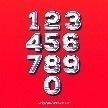
\includegraphics[width=.15\textwidth]{media/image239.jpg}

\item 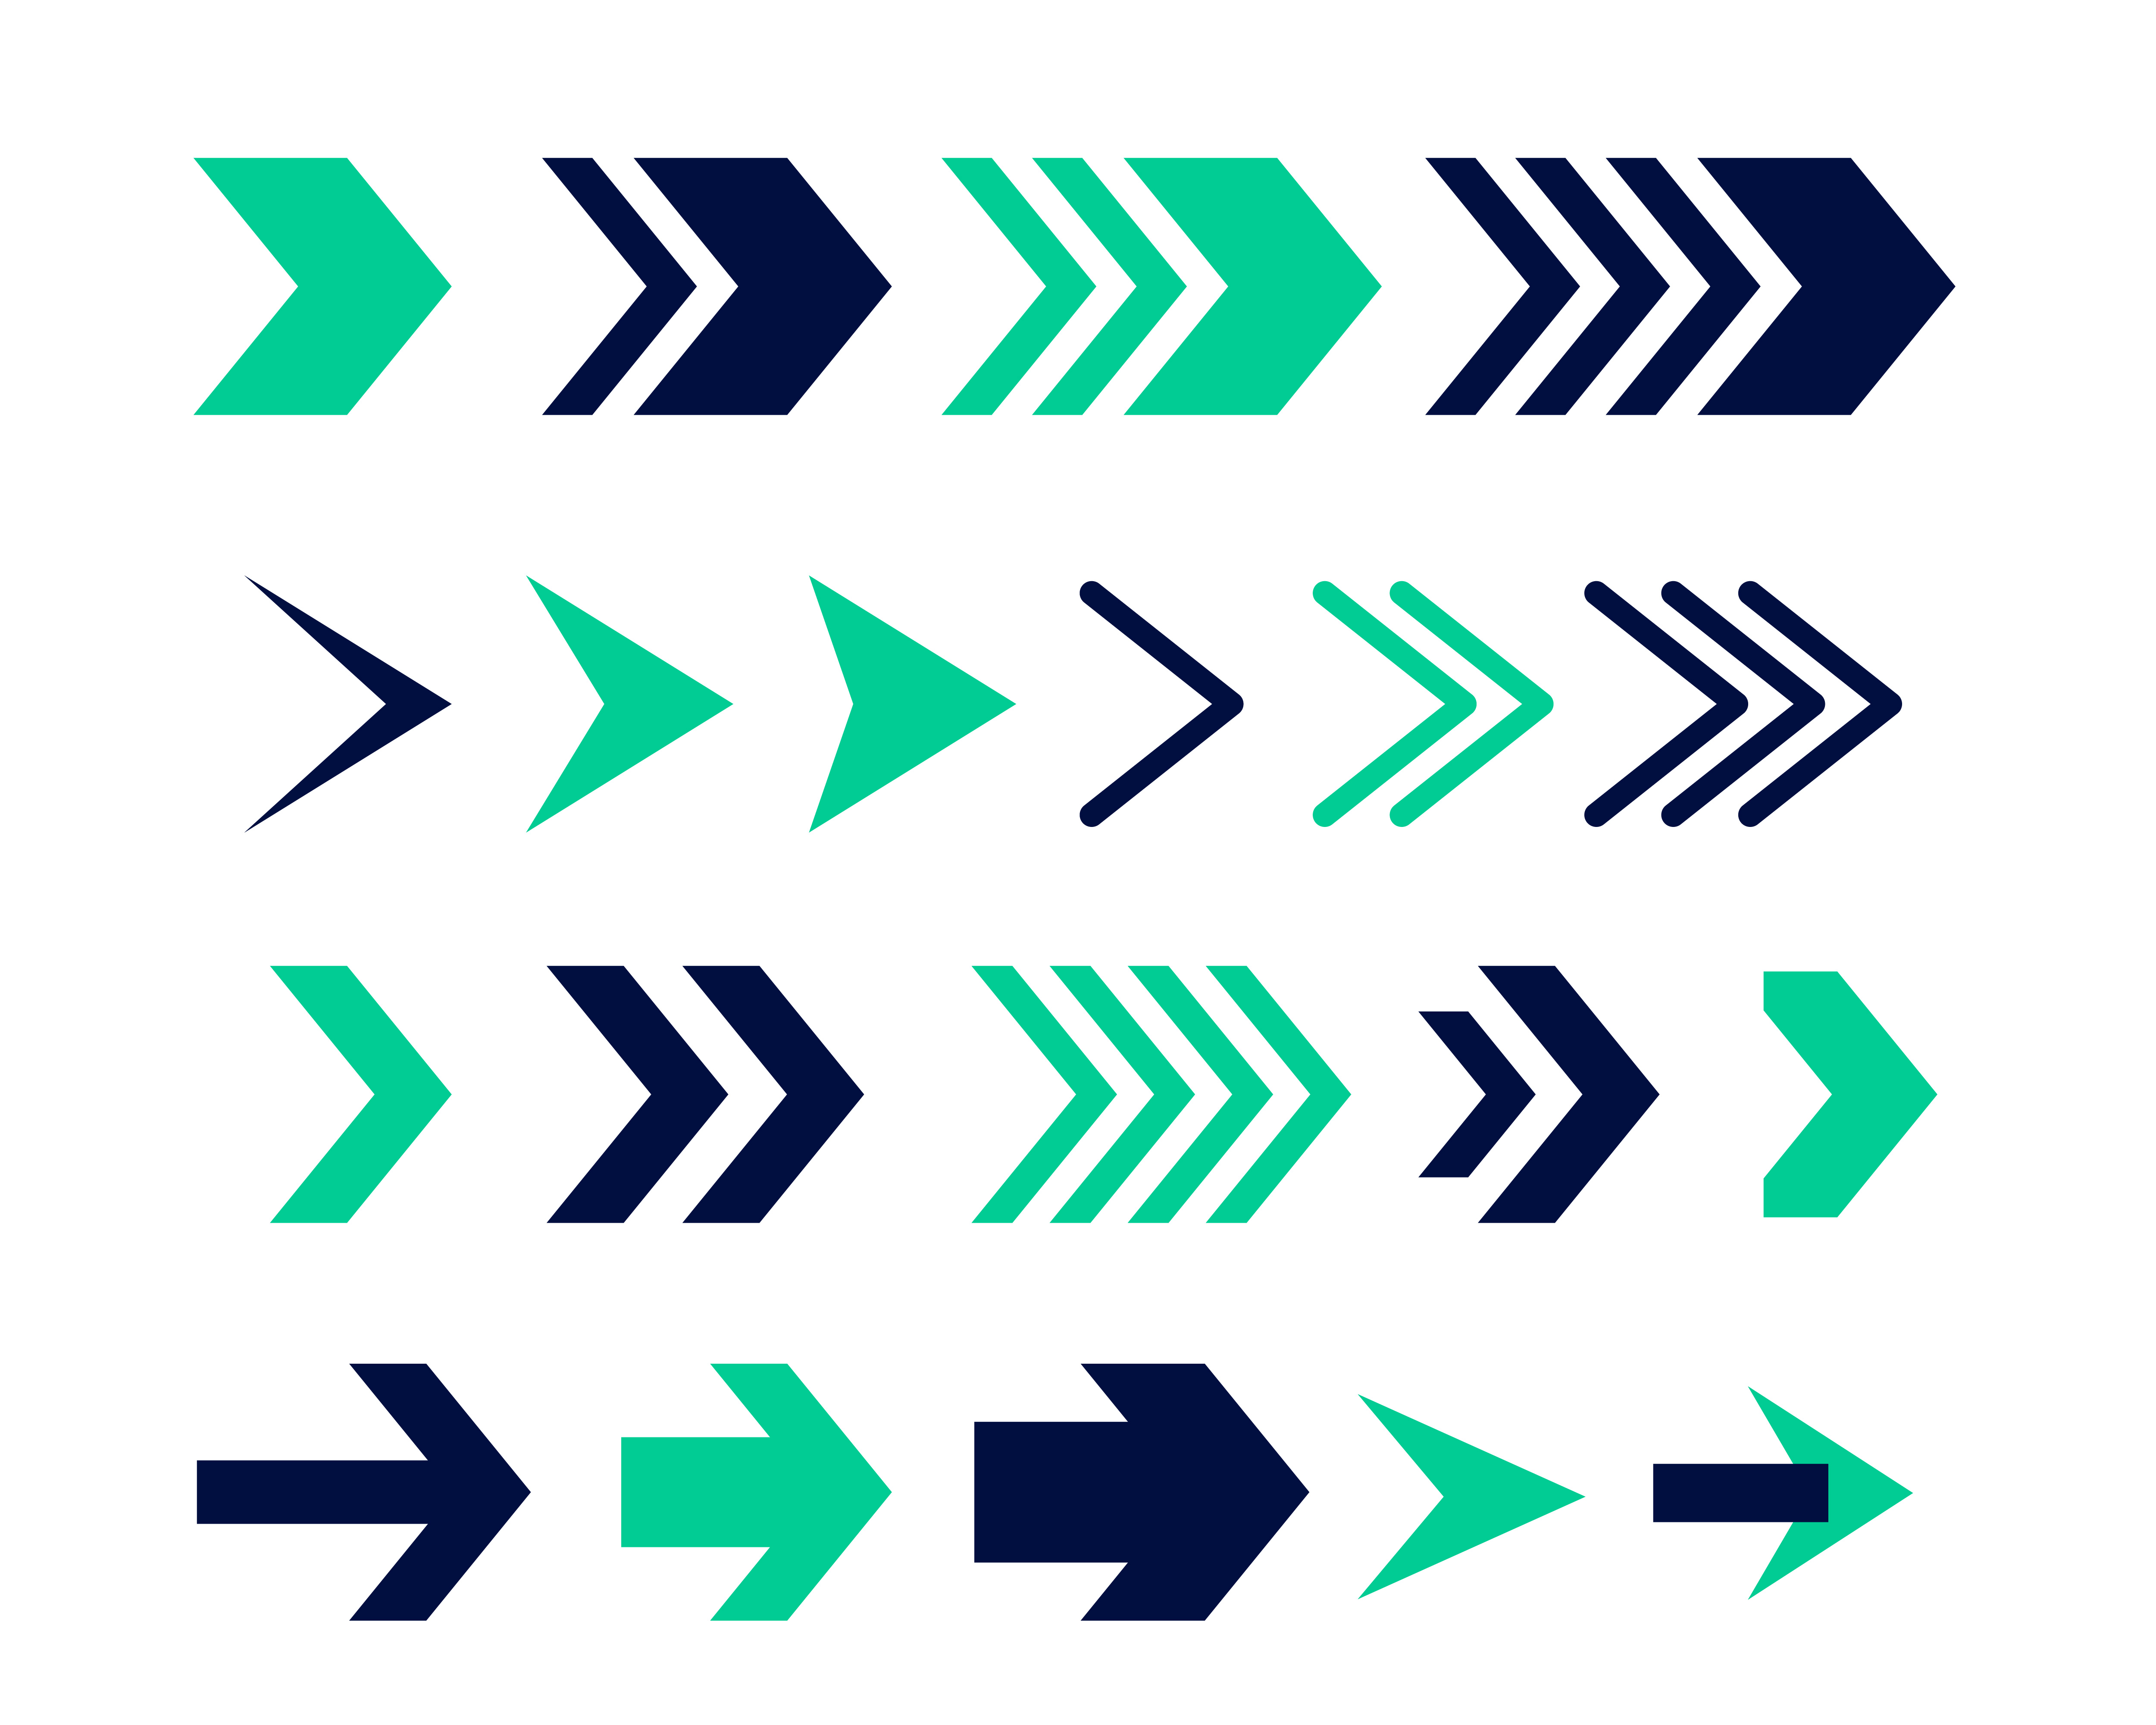
\includegraphics[width=.15\textwidth]{media/image240.jpg}

\item 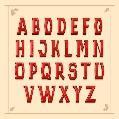
\includegraphics[width=.15\textwidth]{media/image241.jpg}

\item 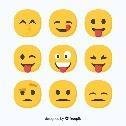
\includegraphics[width=.15\textwidth]{media/image242.jpg}
\end{escolha}

\num{2} VEJA A PALAVRA QUE MARIA ESCREVEU.

\begin{myquote}
SALADA
\end{myquote}

AS LETRAS QUE FORMAM O SOM FINAL DA PALAVRA SÃO

\begin{escolha}
\item D+A.

\item L+A.

\item S+A.

\item A+D.
\end{escolha}

\pagebreak
\num{3} VEJA A PALAVRA QUE DINO CONSEGUIU ESCREVER.

\begin{myquote}
BORBOLETA
\end{myquote}

A PALAVRA QUE TEM A MESMA QUANTIDADE DE SONS QUE ESSA PALAVRA É 

\begin{escolha}
\item BICICLETA.

\item PATINETE.

\item PATINS.

\item BONÉ.
\end{escolha}

\num{4} VEJA A PALAVRA QUE ISA ENCONTROU NO SEU LIVRO. 

\begin{myquote}
JANELA
\end{myquote}

A PALAVRA QUE TEM A MESMA SÍLABA INICIAL DA PALAVRA QUE ISA ENCONTROU É

\begin{escolha}
\item NEVE.

\item JACARÉ.

\item PANELA.

\item LARANJA.
\end{escolha}

\pagebreak
\num{5} VEJA O BRINQUEDO QUE ENZO GANHOU.

\begin{figure}[htpb]
\centering
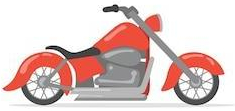
\includegraphics[width=.3\textwidth]{media/image245.jpg}
\end{figure}

%https://www.freepik.com/vectors/motorcycle\#referrer=detail\&resource=11672041

A PALAVRA QUE NÃO APRESENTA NENHUM DOS SONS DO NOME DO BRINQUEDO DE ENZO É

\begin{escolha}
\item FADA.

\item GATO.

\item MOLA.

\item RATO.
\end{escolha}

\num{6} LEIA A ADIVINHAÇÃO. 

\begin{quote}
\begin{verse}
COM DEZ PATAS VAI DE LADO,\\
CONSTELAÇÃO TEM SEU NOME,\\
NÃO TEM PESCOÇO E É CAÇADO\\
PORQUE É GOSTOSO E SE COME.
\end{verse}

\fonte{Domínio Público. ADIVINHAS, CANÇÕES, CANTIGAS DE RODA, PARLENDAS, POEMAS, QUADRINHAS E TRAVA-LÍNGUAS. Disponível em: \emph{https://bit.ly/2svTEzT}. Acesso em 14 abr. 2023. }
\end{quote}

A PRIMEIRA PALAVRA DESSE TEXTO É

\begin{escolha}
\item COM.

\item LADO.

\item COME.

\item POR QUE.
\end{escolha}

\pagebreak
\num{7} OBSERVE ANIMAL DE ESTIMAÇÃO QUE LETÍCIA GANHOU.

\begin{figure}[htpb]
\centering
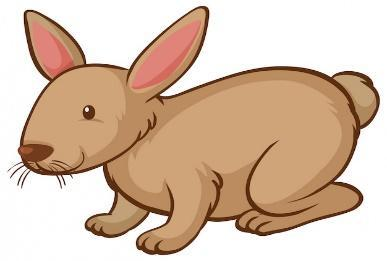
\includegraphics[width=.5\textwidth]{media/image246.jpg}
\end{figure}

O NOME CORRETO DESSE ANIMAL É

\begin{escolha}
\item LHOECO

\item COOLHO.

\item EOCLHO.

\item COELHO.
\end{escolha}

\num{8} LEIA A PALAVRA QUE CATARINA ESCREVEU.

\begin{myquote}
MACACO
\end{myquote}

A PALAVRA QUE COMEÇA COM O SOM IGUAL À PALAVRA QUE ELA ESCREVEU É 

\begin{escolha}
\item NABO.

\item CANECA.

\item COCADA.

\item MACARRÃO.
\end{escolha}

\coment{}

\num{9} SARA GANHOU UM TELE\_\_NE DA SUA TIA. ASSINALE A SÍLABA QUE COMPLETA CORRETAMENTE A PALAVRA.

\begin{escolha}
\item CO

\item PA.

\item FO.

\item FA.
\end{escolha}

\num{10} LEIA A FRASE A SEGUIR.

\begin{myquote}
OS PATOS NADAM NO LAGO.
\end{myquote}

QUAL DESENHO REPRESENTA ESSA FRASE?

\begin{escolha}
\item 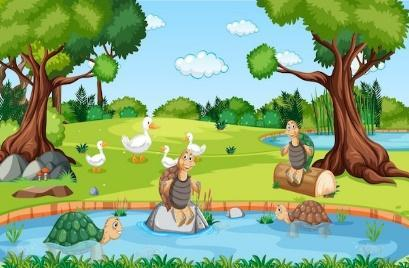
\includegraphics[width=.25\textwidth]{media/image250.jpg}

\item 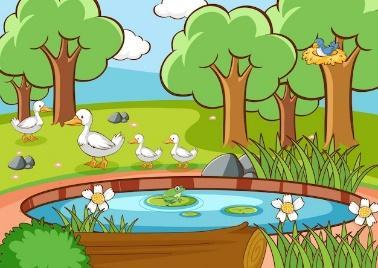
\includegraphics[width=.25\textwidth]{media/image251.jpg}

\item 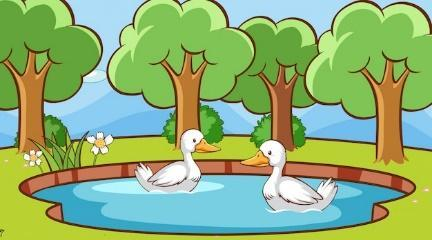
\includegraphics[width=.25\textwidth]{media/image252.jpg}

\item 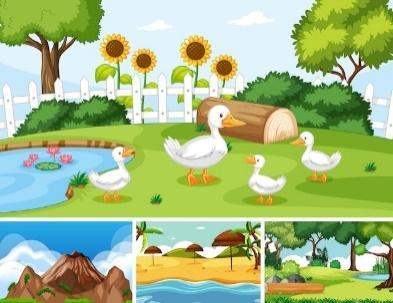
\includegraphics[width=.25\textwidth]{media/image253.jpg}
\end{escolha}


\num{11}

\begin{quote}
\begin{verse}
\textbf{POMBINHA}

POMBINHA QUANDO TU FORES\\
ME ESCREVA PELO CAMINHO\\
SE NÃO ACHARES PAPEL\\
NAS ASAS DE UM PASSARINHO.

DO BICO FAZ UM TINTEIRO\\
DA LÍNGUA PENA DOURADA\\
DOS DENTES LETRA MIÚDA\\
DOS OLHOS CARTA FECHADA.

A POMBINHA VOOU, VOOU {[}BIS{]}\\
FOI-SE EMBORA E ME DEIXOU\\
O QUE A POMBINHA VAI FAZER DOS OLHOS?
\end{verse}
\end{quote}

\begin{escolha}
\item TINTEIRO.

\item LETRA MIÚDA.

\item CARTA FECHADA.

\item PENA DOURADA.
\end{escolha}


\num{12} LEIA O TRECHO DA HISTÓRIA.

\begin{quote}
\textbf{CHAPEUZINHO VERMELHO}

ERA UMA VEZ, NUMA PEQUENA CIDADE ÀS MARGENS DA FLORESTA,
UMA MENINA DE OLHOS NEGROS E LOUROS CABELOS CACHEADOS, TÃO.
GRACIOSA QUANTO VALIOSA.
\end{quote}

\begin{quote}
UM DIA, COM UM RETALHO DE TECIDO VERMELHO, SUA MÃE
COSTUROU PARA ELA UMA CURTA CAPA COM CAPUZ; FICOU UMA
BELEZINHA, COMBINANDO MUITO BEM COM OS CABELOS LOUROS E
OS OLHOS NEGROS DA MENINA.

\fonte{
Disponível em: http://www.dominiopublico.gov.br/download/texto/me001614.pdf. Acesso em: 21 fev. 2023. }
\end{quote}

ESSE TEXTO É DESTINADO ÀS/AOS 

\begin{escolha}
\item JOVENS.

\item CRIANÇAS.

\item ADULTOS.

\item FAMÍLIAS.
\end{escolha}

\num{13} LEIA O TEXTO.

\begin{quote}
\textbf{NO REINO DAS LETRAS FELIZES}

NUM LUGAR MUITO DISTANTE, EXISTIA UM REINO SILENCIOSO, HABITADO APENAS
POR LETRAS, ELAS ERAM MUITO DESUNIDAS. VIVIA CADA UMA PARA SI, E NUNCA
SE REUNIAM PARA FORMAR UMA PALAVRA SEQUER.\textbf{~}A RAINHA ENTÃO
RESOLVEU ACABAR COM AQUELE SILÊNCIO, AQUELE SILÊNCIO TODO, CHAMOU SEUS
CONSELHEIROS: BETA, GAMA E ÔMEGA E ORDENOU:

~-- QUERO QUE ORGANIZEM UM GRANDE BAILE E QUE CONVIDEM TODAS AS LETRAS
DO REINO E TAMBÉM OS DEMAIS REINOS.
\end{quote}

\begin{quote}
A RAINHA TAMBÉM DISSE:

-- QUERO QUE AS LETRAS DO REINO USEM A CRIATIVIDADE E FAÇAM ALGUMAS
APRESENTAÇÕES A FIM DE MARCAR PARA SEMPRE A HISTÓRIA DO REINO.

\fonte{\emph{Disponível em: http://www.dominiopublico.gov.br/pesquisa/DetalheObraDownload.do?select\_action=\&co\_obra=53489\&co\_midia=}
Acesso em: 21 fev. 2023.}
\end{quote}

DE QUE FALA O TEXTO?

\begin{escolha}
\item A APRESENTAÇÃO DAS LETRAS.

\item O SILÊNCIO DAS LETRAS.

\item A TRISTEZA DAS LETRAS. 

\item A ALEGRIA DAS LETRAS.
\end{escolha}

\num{14} LEIA.

\begin{quote}
\textbf{O GALO E A RAPOSA}

O GALO E AS GALINHAS VIRAM QUE LÁ LONGE VINHA UMA RAPOSA.

EMPOLEIRARAM-SE NA ÁRVORE MAIS PRÓXIMA, PARA ESCAPAR DA INIMIGA.

COM SUA ESPERTEZA, A RAPOSA CHEGOU PERTO DA ÁRVORE E
SE DIRIGIU A ELES:
\end{quote}

\pagebreak
\begin{quote}
--- ORA, MEUS AMIGOS, PODEM DESCER DAÍ. NÃO SABEM QUE
FOI DECRETADA A PAZ ENTRE OS ANIMAIS? DESÇAM E VAMOS FESTEJAR ESSE
DIA TÃO FELIZ!

\fonte{Domínio Público. ADIVINHAS, CANÇÕES, CANTIGAS DE RODA, PARLENDAS, POEMAS, QUADRINHAS E TRAVA-LÍNGUAS. Disponível em: \emph{http://www.dominiopublico.gov.br/download/texto/me001614.pdf}. Acesso em 14 abr. 2023.}
\end{quote}

A RAPOSA QUERIA QUE O GALO E A GALINHA DESCESSEM DA ÁRVORE PARA

\begin{escolha}
\item FAZER UMA FESTA.

\item COMÊ-LOS.

\item BRINCAR COM ELES.

\item CONTAR UM SEGREDO.
\end{escolha}

\num{15} LEIA O DIÁLOGO. %E OBSERVE A IMAGEM.

%Paulo: Inserir imagem disponível no link: https://br.freepik.com/fotos-gratis/retrato-de-duas-irmas-afro-americanas-sorridentes_6873868.htm#page=2&query=boy%20giving%20girl%20a%20gift&position=8&from_view=search&track=ais.

%Disponível em: https://br.freepik.com/fotos-gratis/retrato-de-duas-irmas-afro-americanas-sorridentes_6873868.htm#page=2&query=boy%20giving%20girl%20a%20gift&position=8&from_view=search&track=ais. Acesso em: 19 abr. 2023.

\begin{quote}
— TENHO UMA SURPRESA PARA VOCÊ, JULIANA.

— O QUE É, MAMÃE?

— UM PRESENTE!

— OH! MUITO OBRIGADA!
\end{quote}

JULIANA ESTÁ FELIZ PORQUE

\begin{escolha}
\item FOI VIAJAR.

\item GANHOU UM PRESENTE DE SUA MÃE.

\item ESTÁ BRINCANDO COM SEU GATINHO.

\item ESTÁ JOGANDO BOLA.
\end{escolha}


